\documentclass[a4paper]{article} % papier A4
\usepackage[utf8]{inputenc}      % accents dans le source
\usepackage[T1]{fontenc}         % accents dans le pdf
\usepackage{textcomp}            % symboles complémentaires (euro)
\usepackage[frenchb]{babel}      % titres en français
\usepackage{amsmath}
\usepackage{amsthm}
\usepackage{amssymb}
\usepackage[colorlinks=false]{hyperref} %Apparemment ça sert à rien...
\usepackage{enumerate}
\usepackage{tocloft}             % Pour la table des matières
\usepackage{algorithm}
\usepackage{algorithmic}
\usepackage{pgf}
\usepackage{tikz}
\usepackage{tikz-cd}
\usepackage{rotating}
\usetikzlibrary{matrix,arrows,decorations.pathmorphing}
\usepackage{array}
\usepackage{caption}
\usepackage{graphicx}

% Numérotation des sections, sous-sections, équations, etc.
\numberwithin{section}{part}
\numberwithin{equation}{section}

% Maccros pour les commandes de math
\newcommand\nroot[1]{\textit{#1}-ième}
\newcommand\zmodn[1]{\mathbb{Z}/#1\mathbb{Z}}
\newcommand\zmodninv[1]{(\mathbb{Z}/#1\mathbb{Z})^{\times}}
\newcommand\GF[1]{\mathbb{F}_{#1}}
\newcommand\Irr[2]{\textup{min}_{#1}(#2)}
\newcommand\Tr[1]{\textup{Tr}\left(#1\right)}
\newcommand\QQ{\mathbb{Q}}
\newcommand\ZZ{\mathbb{Z}}
\newcommand\NN{\mathbb{N}}
\newcommand\CC{\mathbb{C}}
\newcommand\RR{\mathbb{R}}
\newcommand\EO{\mathcal{O}}
\newcommand\PP[1]{\mathbb{P}^{#1}}
\newcommand\etmath{\textup{\quad et \quad}}
\newcommand\M[1]{\textup{M}(#1)}
\newcommand\E[1]{\textup{E}(#1)}
\newcommand\I[1]{\textup{I}(#1)}
\newcommand\tO[1]{\widetilde{O}(#1)}
\newcommand\groupgen[1]{\langle{#1}\rangle}
\newcommand\ord[2]{\textup{ord}_{#1}(#2)}
\newcommand{\HRule}{\rule{\linewidth}{0.5mm}}

% Algorithmic en français
\floatname{algorithm}{Algorithme}
\renewcommand{\algorithmicrequire}{\textbf{Entrée :}}
\renewcommand{\algorithmicensure}{\textbf{Sortie :}}
\renewcommand{\algorithmiccomment}[1]{\{#1\}}
\renewcommand{\algorithmicend}{\textbf{fin}}
\renewcommand{\algorithmicif}{\textbf{si}}
\renewcommand{\algorithmicthen}{\textbf{alors}}
\renewcommand{\algorithmicelse}{\textbf{sinon}}
\renewcommand{\algorithmicelsif}{\algorithmicelse\ \algorithmicif}
\renewcommand{\algorithmicendif}{\algorithmicend\ \algorithmicif}
\renewcommand{\algorithmicfor}{\textbf{pour}}
\renewcommand{\algorithmicforall}{\textbf{pour tout}}
\renewcommand{\algorithmicdo}{\textbf{faire}}
\renewcommand{\algorithmicendfor}{\algorithmicend\ \algorithmicfor}
\renewcommand{\algorithmicwhile}{\textbf{tant que}}
\renewcommand{\algorithmicrepeat}{\textbf{répéter}}
\renewcommand{\algorithmicuntil}{\textbf{jusqu'à}}
\renewcommand{\algorithmicreturn}{\textbf{renvoyer}}
\renewcommand{\algorithmicto}{\textbf{à}}

\renewcommand{\listalgorithmname}{Liste des algorithmes}
\renewcommand{\listfigurename}{Liste des figures}



% Éviter l'overlap dans la table des matières pour les sections, sous-sections
% etc.
\setlength{\cftsecnumwidth}{3em}    
\setlength{\cftsubsecnumwidth}{3em} 


\sloppy
\begin{document}
\title{Calcul d'isomorphismes de corps finis}
\author{Ludovic Brieulle}
\newtheorem{thm}{Théorème}[section]
\newtheorem{lem}[thm]{Lemme}
\newtheorem{cor}[thm]{Corollaire}
\newtheorem{prop}[thm]{Proposition}
\newtheorem{conj}[thm]{Conjecture}
\theoremstyle{definition}
\newtheorem{defn}[thm]{Définition}
\newtheorem{defnp}[thm]{Définition et proposition}
\newtheorem*{ex}{Exemple}
\theoremstyle{remark}
\newtheorem*{rem}{Remarque}

\begin{titlepage}
%----------------------------------------------------------------------------------------
%	HEADING SECTIONS
%----------------------------------------------------------------------------------------

\begin{center}
\LARGE Université de Versailles Saint-Quentin-en-Yvelines\\[1.5cm] % Name of your university/college
\Large Mémoire de stage de master 2 d'Algèbre Appliquée au Calcul formel et à la
Cryptographie\\[0.5cm] % Major heading such as course name
\large Effectué au sein de l'Agence Nationale de la Sécurité des
Systèmes d'Information\\[0.5cm] % Minor heading such as course title

%----------------------------------------------------------------------------------------
%	TITLE SECTION
%----------------------------------------------------------------------------------------

\HRule \\[0.4cm]
{ \huge \bfseries Calcul d'isomorphismes de corps finis}\\[0.4cm] % Title of your document
\HRule \\[1cm]
 
%----------------------------------------------------------------------------------------
%	AUTHOR SECTION
%----------------------------------------------------------------------------------------
\end{center}
\begin{minipage}{0.4\textwidth}
\begin{flushleft} \large
\emph{Auteur :}\\
Ludovic \textsc{Brieulle} % Your name
\end{flushleft}
\end{minipage}
\begin{minipage}{0.5\textwidth}
\begin{flushright} \large
\emph{Encadré par :} \\
Luca \bsc{De Feo} (PRiSM, UVSQ)\\ % Supervisor's Name
Jean-Pierre \bsc{Flori} (ANSSI)\\% Supervisor's Name
Jérôme \bsc{Plût} (ANSSI)\\% Supervisor's Name
\end{flushright}
\end{minipage}\\[1cm]

% If you don't want a supervisor, uncomment the two lines below and remove the
% section above
%\Large \emph{Author:}\\
%John \textsc{Smith}\\[3cm] % Your name

%----------------------------------------------------------------------------------------
%	DATE SECTION
%----------------------------------------------------------------------------------------

\begin{center}
{\large 16 septembre 2014}\\[1cm] % Date, change the \today to a set date if you want to be
\end{center}

%----------------------------------------------------------------------------------------
%	LOGO SECTION
%----------------------------------------------------------------------------------------

\begin{center}

\includegraphics[width=9cm]{136704} % Include a department/university logo - this

\includegraphics[width=9cm, height=2.7cm]{uvsq-logo-rvb-def}\\
\end{center}
 
%----------------------------------------------------------------------------------------

\vfill % Fill the rest of the page with whitespace
\end{titlepage}
\newpage

\part*{Introduction}
\addcontentsline{toc}{part}{Introduction}
Soit $p$ un nombre premier et soit $\GF{q}$ le corps fini à $q = p^r$ éléments. 
Il est connu que deux corps finis de même cardinal sont reliés par un 
isomorphisme. Cependant la preuve de ce résultat ne permet pas d'expliciter
efficacement un tel isomorphisme, le trouver demande alors un travail 
supplémentaire. La situation est la suivante, on a deux extensions de 
$\GF{q}$ de même degré et définies par deux polynômes irréductibles distincts 
$f$ et $g$. On notera :
\[k_1=\GF{q}[X]/(f)\etmath k_2=\GF{q}[Y]/(g)\]
le but est donc de trouver un isomorphisme reliant ces deux corps.\par
Une méthode simple et immédiate est d'envoyer $x = \bar{X}$ la classe de $X$
dans $k_1$, sur une racine de $f$ dans $k_2$. Le problème est que cela revient à
factoriser le polynôme $f$ ce qui en pratique demande beaucoup de temps. On 
étudiera dans ce mémoire l'algorithme de Rains \cite{Rai}, amélioration d'une 
idée de Pinch \cite{Pin}, pour déterminer des isomorphismes de corps finis. Plus
précisément, on énoncera deux variantes de cet algorithme, l'une dite 
cyclotomique et faisant usage des racines de l'unité, l'autre dite elliptique et
faisant usage de points d'ordres finis d'une courbe elliptique sur les corps 
finis. On montrera que toutes ces méthodes ont des complexités proches, l'un des
objectifs de ce mémoire sera donc d'implanter et de comparer ces méthodes en 
pratique.\par
On note aussi l'existence d'une méthode établie par Allombert \cite{All} qui 
consiste à utiliser l'algèbre linéaire pour déterminer un isomorphisme, donc une
complexité en $O(n^{\omega})$ avec $2<\omega<3$ et $n$ le degré de l'extension
traitée.\par
\newpage

\part*{Remerciements}
Je tiens tout d'abord à remercier l'\bsc{ANSSI} (Agence Nationale de la Sécurité
des Systèmes d'Informations) pour m'avoir accueilli, le cadre de travail de 
l'agence et l'ambiance des locaux ont grandement participé au bon déroulement de
mon travail durant ces six mois de stage.\par
Je remercie aussi mes encadrants, Jérôme Plût (ANSSI), pour nos brèves mais
enrichissantes divergences mathématiques; Luca De Feo (UVSQ), pour m'avoir 
accueilli à l'UVSQ et pour les nombreux conseils et pistes qui m'ont permis
d'avancer; Jean-Pierre Flori (ANSSI) pour ses conseils tout au long du stage,
pour la liberté qu'il m'a donné et pour m'avoir initié à la marche à pied. 
Je tiens à les remercier collectivement pour m'avoir permis de participer, bien 
que très modestement, à leur projet de recherche. Grâce à eux j'ai pu rencontrer
plusieurs membres du milieux de la cryptographie et participer à plusieurs
rencontres intéressantes, notamment les sagedays.\par
Je tiens aussi à remercier mes collègues de l'ANSSI Théo, Tom et Maxime, sans qui
ces six mois de stage n'auraient pas été les mêmes, sans qui être assis sur 
l'herbe en bord de Seine et au soleil aurait été bien ennuyeux. Je salue 
aussi mes collègues du master MA2CC, Nicolas, Ivan, Chloé, Sébastien, Riad et 
Ngo, notamment ceux que j'ai pu rencontrer pendant mon stage.
\newpage

\tableofcontents
\listoffigures
\listofalgorithms
\listoftables
\newpage

\part{Rappels et contexte théorique}
\label{un}

Cette partie consiste principalement à rappeler et énoncer les résultats
nécessaires pour la suite. Cette partie n'a pas pour vocation de faire un exposé
complet des notions abordées, pour un traité plus 
détaillé, le lecteur pourra consulter au choix \cite{LiNi1} ou 
\cite[chap.~III]{Per} pour les corps finis; \cite[chap.~VI]{Sam}, \cite{Lan1} ou
\cite{Esc} pour la théorie de Galois; \cite{Sam} ou \cite{Lan2} pour la théorie 
des nombres; \cite{Sil} ou \cite{Was2} pour la théorie sur les courbes 
elliptiques; et pour finir \cite{GaGe} pour tout ce qui concerne le calcul 
formel en général. On s'efforcera néamoins de démontrer les résultats les plus 
importants. Le c\oe{}ur du sujet se trouve lui dans les parties \ref{deux} et 
\ref{trois}.

\section{Corps finis}
Dans cette section on rappelle les définitions et démontre certains 
résultats liés aux corps finis. Principalement, on exposera les notions de bases
d'extensions de corps et la théorie de Galois sur les corps finis. 
Tous les corps sont considérés commutatifs. On notera $(a,b)$ le pgcd entre deux
entiers $a$ et $b$.


\subsection{Extension de corps}
\label{def:degext}
Soient $k$ et $K$ deux corps, s'il existe un homomorphisme de $k$ vers $K$ alors
celui-ci est nécessairement injectif. On dit que $K$ est une extension de corps 
de $k$ s'il existe un morphisme de corps $\varphi : k \to K$ ou de façon 
équivalente, si $k \subseteq K$ alors $K$ est une extension (de corps) de $k$. 
On notera $K/k$ une extension de corps. Si on a $k\subseteq L \subseteq K$, 
alors $L/k$ est une sous-extension de $K/k$. On appelle corps premier un corps 
qui n'a pas de sous-corps ou de sous-extensions.\par
Soit $K/k$ une extension de corps et soit $S$ une partie de $K$. Le sous-corps 
$L := k(S)$ de $K$ engendré par $S$ sur $k$ est le plus petit sous-corps de $K$ 
contenant $S$ et $k$. Si $S = \lbrace x_1,\dots,x_n \rbrace$ est fini, alors on 
note $L = K(x_1,\dots,x_n)$, on dit alors que l'extension est de \emph{type
fini}. L'extension $L/k$ est dite \emph{monogène} ou \emph{simple} si elle est
engendrée par un seul élément. Si $K/k$ est une extension de corps, on peut
alors voir $K$ comme un $k$-espace vectoriel ou une $k$-algèbre. On appelle 
$[K:k] := dim_k(K)$ le \emph{degré} de l'extension. On dit qu'une extension 
$K/k$ est de degré fini si $[K:k] < \infty$.\par

\begin{thm}
Soient $k \subseteq L \subseteq K$ des extensions de corps de degré fini. Alors 
on a :
\begin{equation}
[K:k] = [K:L][L:k].
\end{equation}
\end{thm}
\begin{proof}
On pose $[K:L] = m$ et $[L:k] = n$. On a donc que $K$ est un $L$-espace 
vectoriel de dimension $m$ et $L$ est un $k$-espace vectoriel de dimension $n$, 
le théorème revient à montrer que $K$ est un $k$-espace vectoriel de dimension 
$mn$. Or, d'après ce qui précède, on a $L \simeq k^n$ et $K \simeq L^m$, d'où
\begin{equation}
K \simeq \underbrace{L \oplus\dots\oplus L}_{m fois}\simeq\underbrace
{k^n\oplus\dots\oplus k^n}_{m fois} \simeq k^{nm},
\end{equation}
ce qui prouve le théorème.
\end{proof}

On dit qu'un élément $x\in K$ est \emph{algèbrique} sur $k$ s'il existe un 
polynôme unitaire à coefficients dans $k$ qui annule $x$. L'ensemble des 
éléments algébriques d'un corps (sur un sous-corps) forme un corps \cite[p.~64, 
théorème 1.14]{Per}. On dit qu'une extension $K/k$ est algébrique si tous les 
éléments de $K$ sont algébriques sur $k$. En particulier, toute extension de
degré fini est algébrique et de type fini.\par
Soit $L/K$ une extension de corps et soit $\alpha\in L$ un élément algébrique 
sur $K$. Si on note $\Irr{K}{\alpha}$ le \emph{polynôme minimal} de $\alpha$ sur
$K$ et on pose $n := \textup{deg\,}\Irr{K}{\alpha}$ alors l'anneau des polynômes
sur $K$ en $\alpha$ noté $K[\alpha]$ est égal au corps des fractions rationnels
en $\alpha$, $K(\alpha)$ et c'est un $K$-espace vectoriel de dimension de $n$.
\begin{defnp}
Soit $K(\alpha)/K$ une extension monogène, alors les éléments 
$1,\alpha,\dots,\alpha^{n-1}$ forment une base de $K(\alpha)$ en tant que
$K$-espace vectoriel et on l'appelle la \emph{base monomiale}.
\end{defnp}
\begin{proof}
Voir \cite[III, th. 1.11]{Per}.
\end{proof}

En résumé, $K(\alpha)/K$ est une extension de corps de
degré $n$, on l'appelle le \emph{corps de rupture} de $\Irr{K}{\alpha}$ et
s'obtient en quotientant l'anneau des polynômes sur $K$ par l'idéal engendré par
le polynôme minimal de $\alpha$. De façon plus générale, le corps de rupture 
d'un polynôme $P$ dans $K[X]$ est l'extension de $K$ obtenue en adjoignant une 
racine $\alpha$ de $P$ à $K$ :
\begin{equation}
K(\alpha)\simeq K[X]/(P).
\end{equation}

Considérons une extension $L/K$ telle que $P\in K[X]$ irréductible admette une 
racine $\alpha\in L$. Alors $\Irr{K}{\alpha}$ divise $P$, donc est égal à 
$\lambda P$ pour $\lambda\in K^{\times}$, puisque $P$ est irréductible. Alors 
le morphisme de $K$-algèbres $\phi : K[X] \to L$ défini par $\phi(X) = \alpha$ 
induit un morphisme de $K$-algèbre $\varphi : K[X]/(P) \to L$ tel que 
$\varphi(x) = \alpha$. Ce morphisme est unique puisque $x$ engendre $K[X]/(P)$. 
Ce qui montre en particulier l'existence et l'unicité à isomorphisme près des 
corps de rupture.\par
\vspace{0.3cm}
Une autre notion importante est celle de corps de décomposition d'un polynôme 
non constant sur un corps $k$.

\begin{defn}
\label{def:dec}
Soit $K$ un corps et soit $\overline{K}$ une clôture algébrique de $K$. On 
appelle corps de décomposition de $P\in K[X]$, le corps $L\subset\overline{K}$ 
tel que $P$ soit scindé dans $L$ et que ses racines engendrent $L$ sur $K$.
\end{defn}

\begin{thm}
\label{cor:dec}
Tout $P\in K[X]$ non constant admet un corps de décomposition unique à 
isomorphisme près.
\end{thm}
\begin{proof}
    Voir \cite[Chap III, th. 1.30]{Per}.
\end{proof}



%TODO : Trace, norme, multiplication par un élément ? Non dégénérescence de Tr ?

Deux notions importantes pour les extensions de corps sont la trace et la norme
d'un élément d'une extension par rapport à un sous-corps. On les définit comme
suit:

\begin{defnp}
Soit un $K$ un corps de caractéristique 0 ou fini et soit $L/K$ une extension
algébrique de degré $n$ sur $K$. Soient $x_1,\dots, x_n$ les racines du polynôme
minimal de $x$, dans le corps de décomposition de celui-ci, chacune répétée 
$[L:K(x)]$ fois; alors on a :
\begin{equation}
Tr_{L/K}(x) = x_1 + \dots + x_n \etmath N_{L/K}(x) = x_1\dots x_n.
\end{equation}
De plus, le polynôme caractéristique de $x$ relativement à $L$ et $K$ est $(X -
x_1)\dots(X - x_n)$.
\end{defnp}
\begin{proof}
Voir \cite[p. 44, prop. 1]{Sam}.
\end{proof}
%TODO: La preuve, éventuellement.
%TODO: Je voulais en déduire que la trace est surjective, mais je sais plus trop
%comment, si tu t'en souviens un jours...
\subsection{Notions de théorie de Galois}
%TODO :Définitions et résutlats de base (sans forcément tout prouver),
%Frobenius, action de groupes ? Ça me parait raisonnable...
%Groupe de Galois, élément primitif, extensions galoisiennes, etc.
Soit un corps $L$ et soit l'ensemble $G$ des automorphismes de $L$. L'ensemble 
des éléments de $x\in L$ tels que $\sigma(x) = x$ pour tout $\sigma\in G$ est un
sous-corps $K$ de $L$, c'est le corps des invariants de $G$. Soient $L/K$ et
$L'/K$ deux extensions de corps, on appelle $K$-homomorphismes de $L$ dans $L'$ 
les morphismes de $K$-algèbres de $L$ dans $L'$. Si $L = L'$ alors on parle de
$K$-automorphisme et ceux-ci forment un groupe pour la loi de composition.

\begin{thm}
\label{th:defgal}
Soit $L/K$ une extension de corps de type fini de degré $n$, avec $K$ un corps
fini ou de caractéristique nulle. Les conditions suivantes sont équivalentes :
\begin{enumerate}[(i)]
	\item $K$ est le corps des invariants du groupe $G$ des $K$-automorphismes
de $L$.
	\item Pour tout $x\in L$, le polynôme minimal de $x$ sur $K$ a toutes ses
racines dans $L$.
	\item $L$ est engendré par les racines d'un polynôme sur $K$.
\end{enumerate}
Dans ces conditions, le groupe $G$ est d'ordre égal à $n$.
\end{thm}
\begin{proof}
Voir \cite[p. 101, th. 1]{Sam}.
\end{proof}

\begin{defn}
\label{def:gal}
Une extension de corps est une \emph{extension galoisienne} si elle satisfait 
les conditions du théorème \ref{th:defgal}. Dans ce cas, $G$ s'appelle le groupe
de Galois de $L/K$, on le note $G := Gal(L/K)$. Si $G$ est abélien (resp. 
cyclique) alors l'extension est dite abélienne (resp. cyclique).
\end{defn}

Un polynôme irréductible $f$ est \emph{séparable} sur un corps $K$ si toutes
ses racines dans un corps de décomposition sont distinctes; la notion est
indépendante du corps de décomposition choisi, puisqu'il existe un $K$-morphisme
reliant les racines et dans ce cas leurs images sont aussi distinctes. 
Un élément $\alpha$ est \emph{séparable} sur $K$ si son polynôme minimal est 
séparable sur $K$.

\begin{defn}
\label{def:sep}
Une extension algébrique $L/K$ est \emph{séparable} si tous les $\alpha\in L$
sont séparables.
\end{defn}

\begin{rem}
On peut définir la séparabilité d'un polynôme réductible en se basant sur ses
facteurs irréductibles, un polynôme sera séparable si tous ses facteurs
irréductibles le sont.
\end{rem}

\begin{prop}
\label{prop:sepderiv}
Soit $P$ un polynôme sur un corps $K$, on a l'équivalence suivante 
:
\begin{equation}
    P\textup{ séparable } \Leftrightarrow (P', P) = 1.
\end{equation}
\end{prop}
\begin{proof}
    Voir \cite[p. 178]{Lan1}.
\end{proof}

Soit $f$ un polynôme irréductible de degré $n$ sur un corps $K$. Soit $\alpha_1 
:= \alpha$ une racine de $f$ et $\alpha_2,\dots,\alpha_n$ les autres racines de 
$f$ dans un corps de décomposition. Alors on dit que les $\alpha_i$ sont les 
conjugués de $\alpha$ sur $K$.
\begin{defn}
Une extension $L/K$ est \emph{normale} ou \emph{quasi-galoisienne}, si pour tout
$\alpha\in L$, $\Irr{k}{\alpha}$ a toutes ses racines dans $L$ ou, de façon 
équivalente, si $L$ contient tous les conjugués de $\alpha$.
\end{defn}

\begin{prop}
\label{prop:decompnorm}
Soit $P\in k[X]$ de degré $n\geq 1$ et soit $K$ un corps de décomposition de $P$
sur $k$. Alors $K/k$ est normale.
\end{prop}

On peut désormais énoncer un résultat qui permet de déterminer de façon plus
pratique si une extension est galoisienne ou non.

\begin{thm}
Soit $K/k$ une extension de degré fini. Les conditions suivantes sont
équivalentes :
\begin{enumerate}
\item L'extension $K/k$ est galoisienne.
\item L'extension $K/k$ est normale et séparable.
\item Le corps $K$ est le corps de décomposition d'un polynôme séparable.
\end{enumerate}
Sous ces conditions, pour tout $\alpha\in K$ on a :
\begin{equation}
\Irr{k}{\alpha} = \prod_{\beta\in G\alpha}{(X - \beta)}.
\end{equation}
où $G\alpha$ est l'orbite de $\alpha$ sous l'action de $G$.
\end{thm}

\begin{rem}
En particulier, on définit le groupe de Galois d'un polynôme $P$ comme le
groupe de Galois du corps de décomposition de $P$, alors si $P$ est
irréductible, son groupe de Galois agit transitivement sur ses racines.
\end{rem}

\begin{defn}
\label{def:elemnorm}
Soit $L/K$ une extension galoisienne. On dit que $x\in L$ est un élément
\emph{normal} de $L$ si son orbite sous l'action du groupe de Galois forme une 
base de $L$ en tant que $K$-espace vectoriel; ou encore si ses conjugués forment
une base de $L$ en tant que $K$-espace vectoriel. On appelera cette base la 
\emph{base normale} de $L$.
\end{defn}

\begin{thm}
Soit $L/K$ une extension galoisienne, alors il existe une base normale.
\end{thm}
\begin{proof}
Voir \cite[th. 3.72]{LiNi1}.
\end{proof}

\subsection{Définitions}
Soit $p$ un nombre premier, un corps fini $K$ est un corps à $q = p^r$ éléments,
avec $r\geq1$. Le nombre $p$ s'appelle la \emph{caractéristique} du corps $K$ et
vérifie pour tout $x\in K$ :
\begin{equation}
p\cdot x = \underbrace{x+\dots+x}_{p\textup{ fois}} = 0.
\end{equation}
Un corps fini est muni de l'automorphisme de Frobenius défini par :
\begin{equation}
\phi_p : x \mapsto x^p.
\end{equation}
On note :
\begin{equation}
\phi_q = \underbrace{\phi\circ\cdots\circ\phi}_{r\textup{
fois}},
\end{equation}
qui à tout $x\in \bar{K}$ associe $x^q$.\par
On caractérise les éléments de $q$ par l'identité $x^q - x = 0$. En effet, le
groupe des inversibles de $K$ est d'ordre $q-1$, donc pour tout $x\in K$ on a
$x^{q-1} = 1$ et il suffit de multiplier par $x$ pour obtenir l'identité.
On peut complètement caractériser les corps finis par le théorème suivant. Il
assure entre autre que deux corps finis de même cardinal sont isomorphes, ce qui
sera le point de départ de notre travail.

\begin{thm}
\label{th:isomGF}
Pour tout nombre premier $p$ et tout entier strictement positif $r$, il existe 
un corps fini à $p^r$ éléments. Tout corps fini à $q = p^r$ éléments est 
isomorphe au corps de décomposition de $X^q - X$ sur $\GF{p}$. On parlera 
alors du corps fini à $q$ éléments et on le notera $\GF{q}$.
\end{thm}
\begin{proof}
\textit{(Existence)} Pour $q = p^r$, on considère le polynôme $X^q - X$ dans 
$\GF{p}[X]$ et on note $K$ son \emph{corps de décomposition}, définition 
\ref{def:dec}, sur $\GF{p}$. Le polynôme est \emph{séparable}, définition 
\ref{def:sep}, ou n'a aucune racine multiple puisque sa dérivée est égale à 
$qX^{q-1} - 1 = -1$, proposition \ref{prop:sepderiv}. Posons $S=\lbrace x\in K 
: x^q - x = 0\rbrace$, alors $S$ est un sous-corps de $K$; $0$ et $1$ sont 
dans $K$ et d'après les propriétés sur le Frobenius et les résultats obtenus 
plus haut on a :
\begin{equation}
(a - b)^q = a^q - b^q = a - b \etmath(ab^{-1})^q = a^qb^{-q} = ab^{-1}.
\end{equation}
Ainsi, $S$ contient toutes les racines de $X^q - X$ mais comme $K$ a déjà $q$
éléments, alors $K = S$ est un corps à $q$ éléments.\par
\textit{(Unicité)} Soit $K$ le corps à $q = p^r$ éléments, il est de 
caractéristique $p$ et contient $\GF{p}$. On en déduit que $K$ est un corps de 
décomposition de $X^q - X$ sur $\GF{p}$, puisqu'il est scindé sur $K$, et 
l'unicité se déduit de l'unicité des corps de décomposition, corollaire 
\ref{cor:dec}.
\end{proof}

On peut se demander étant donné un corps fini $\GF{p^n}$ quels peuvent être les 
corps qui le contiennent. Dans un premier temps, il faut que les deux corps 
aient la même caractéristique. Supposons qu'il existe un morphisme $f : \GF{p^n}
\to \GF{\ell^m}$ pour $p$ et $\ell$ premiers. En particulier, on a pour 
$x\in\GF{p^n}$ :
\begin{equation}
f(p.x) = 0 = p.f(x),
\end{equation}
pour $f(x)\in\GF{\ell^m}$, donc nécessairement $\ell = p$.\par
Ainsi, si le morphisme existe alors $\GF{p^n}^{\times}$ est un sous-groupe
d'ordre $p^n - 1$ de $\GF{p^m}^{\times}$ d'ordre $p^m - 1$. Donc, on a $p^n - 1$
qui divise $p^m - 1$. Si on écrit $m = q.n + r$ avec $r < n$ alors on obtient :
\[p^m - 1 = p^r((p^n)^q - 1) + p^r - 1\]
Or $p^n - 1$ divise $(p^n)^q - 1$ donc comme $p^n - 1$ divise aussi $p^m - 1$ la
seule possibilité pour $r$ est $0$ et donc $n|m$. On vient de prouver la
nécessité du critère suivant :

\begin{prop}
Soit $\GF{q}$ un corps fini à $q = p^m$ éléments, alors tous ses sous-corps sont
de la forme $\GF{p^n}$ avec $n|m$. Réciproquement, soit $n|m$ alors il existe un
(et un seul) sous-corps de $\GF{q}$ de cardinal $p^n$.
\end{prop}
\begin{proof}
Pour montrer l'autre sens, il suffit de remarquer que $\GF{p^n}$ correspond aux
éléments satisfaisant l'équation $X^{p^n} - X$ puisque $p^n - 1$ divise $p^m -
1$.
\end{proof}

\begin{thm}
\label{th:elemprim}
Toute extension séparable (\ref{def:sep}) et de degré fini est simple.
\end{thm}
\begin{proof}
On va se contenter de le prouver dans le cas d'un corps fini; le cas général
demande un peu plus de travail. On invitera le lecteur à consulter
\cite[p.~87]{Esc}.\par
Si $K$ est un corps fini alors son groupe multiplicatif $K^{\times}$ est
cyclique (voir par exemple la preuve de la proposition \ref{prop:rootcycl} ou
\cite[p.~50]{LiNi1}). Dans ce cas, il suffit de prendre pour générateur d'une
extension $L/k$, le générateur du groupe multiplicatif de $L$.
\end{proof}

Pour les corps finis, déterminer le groupe de Galois est beaucoup plus facile
comme le montre le théorème suivant :

\begin{thm}
Soit $n\geq1$ et soit $\GF{q}$ le corps à $q=p^r$ éléments, avec $p$ premier.
L'extension $\GF{q^n}/\GF{q}$ est galoisienne et son groupe de Galois
$\textup{Gal}(\GF{q^n}/\GF{q})$ est cyclique d'ordre $n$, engendré par 
l'automorphisme de Frobenius $\phi_q$.
\end{thm}
\begin{proof}
On a déjà montré que $\GF{q^n}$ était le corps de décomposition de $Q = X^{q^n} 
- X$, théorème \ref{th:isomGF}, donc que l'extension était normale, proposition 
\ref{prop:decompnorm}. De plus, comme $Q' = -1 \neq 0$, $Q$ est séparable,
proposition \ref{prop:sepderiv}, d'où $\GF{q^n}/\GF{q}$ est galoisienne
et donc :
\[|\textup{Gal}(\GF{q^n}/\GF{q})| = [\GF{q^n}:\GF{q}] = n\]
Comme le Frobenius est un $\GF{q}$-automorphisme, c'est un morphisme et un 
élément de $\GF{q}$ élevé à la puissance $q^n$ est toujours égal à lui-même, 
c'est un élément de $\textup{Gal}(\GF{q^n}/\GF{q})$. Notons $d$ son ordre, alors
$\phi_q^d = Id_{\GF{q^n}}$ ou encore, pour tout $x\in\GF{q^n}$ :
\[\phi_q^d(x) = x^{q^d} = x \Leftrightarrow x^{q^d} - x = 0\]
Le polynôme $X^{q^d} - X$ ayant au plus $d$ racines, on a $d\geq n$ et donc $d =
n$ d'où $\phi_q$ engendre $\textup{Gal}(\GF{q^n}/\GF{q})$ et donc le
résultat.
\end{proof}

%TODO : Groupe de décomposition et groupe d'inertie ?
\subsection{Extensions et polynômes cyclotomiques}
%TODO : Racines de l'unités et quelques mots sur les polynômes 
%cyclotomiques et leurs extensions. Peut-être rajouter un ou deux mots sur le 
%cas des corps finis.
Soit $A$ un anneau et soit $n\in\NN$, une racine \nroot{n} de l'unité dans $A$ 
est un élément $u$ de $A$ tel que $u^n = 1$. On note $\mu_{n,A}$ l'ensemble des 
racines \nroot{n} de l'unité dans $A$ et pour tout corps $K$, on note 
$\mu_{n,\bar{K}}$ l'ensemble des racines de l'unité dans une clôture algébrique 
de $K$. Comme il ne dépend pas du choix de la clôture algébrique, on le note 
$\mu_{n,K}$.\par

\begin{prop}
\label{prop:rootcycl}
L'ensemble $\mu_{n,K}$ forme un groupe pour la multiplication dans $K$ et si 
$|\mu_{n,K}| = n$ alors il est non canoniquement isomorphe à $\zmodn{n}$.
\end{prop}
\begin{proof}
Voir \cite[p. 28, th. 1]{Sam} ou \cite[pp. 177-178]{Lan1}.
\end{proof}

\begin{defn}
On appelle racine \emph{primitive} \nroot{n} un générateur de $\mu_{n,K}$. On 
note $\mu_{n,K}^{\times}$ l'ensemble de ces racines.
\end{defn}

Lorsqu'on les considère sur $\CC$, on définit à partir des racines primitives de
l'unité le polynôme suivant :
\begin{equation}
\Phi_n(X) = \prod_{\zeta\in \mu_n^{\times}}{(X - \zeta)}.
\end{equation}

C'est un polynôme irréductible à coefficients dans $\ZZ$ \cite[prop 4.8]{Per} et
de degré $\varphi(n)$ où $\varphi$ est l'indicatrice d'Euler. On l'appelle 
le \nroot{n} \emph{polynôme cyclotomique}, il s'agit du polynôme minimal des 
racines \nroot{n} de l'unité. Soit $K$ un corps, on appelle 
\emph{extension cyclotomique} de $K$ le corps de décomposition de $\Phi_n$ sur 
$K$.

\begin{rem}
Dans le cas $K = \QQ$, le corps de décomposition de $\Phi_n$ est exactement 
$\QQ(\zeta_n) \simeq \QQ[X]/\phi_n(X)$, où $\zeta_n$ est une racine primitive. 
C'est en particulier une extension algébrique simple.
\end{rem}

Le théorème \ref{th:polycycldecomp} est crucial pour la suite du mémoire, il 
sert notamment à justifier une partie de l'algorithme de Rains cyclotomique.

\begin{thm}
\label{th:polycycldecomp}
Si $K = \GF{q}$ et $(n,q) = 1$, alors $\Phi_n$ se factorise en $\varphi(n)/d$ 
polynômes unitaires irréductibles dans $\GF{q}[X]$ de même degré égal à $d$. Si
on note $K^{(n)}$ le corps de décomposition de n'importe lequel de ces facteurs,
on a :
\[[K^{(n)}:K] = d\]
avec $d$ l'ordre multiplicatif de $q$ dans $\zmodn{n}$.
\end{thm}
\begin{proof}
Voir \cite[th. 2.47]{LiNi1}.
\end{proof}

\begin{prop}
\label{prop:cyclgal}
Soit $n \geq 2$ et soit $\zeta$ une racine primitive \nroot{n} de l'unité sur 
$\QQ$, alors l'extension $\QQ(\zeta_m)/\QQ$ est galoisienne. En particulier :
\begin{enumerate}[(i)]
\item L'extension $\QQ(\zeta_m)/\QQ$ est normale.

\item On a $[\QQ(\zeta_m):\QQ] = \varphi(n)$.

\item Et $\textup{Gal}(\QQ(\zeta_m)/\QQ) = \zmodn{n} \simeq \mu_{n,\QQ}$.
\end{enumerate}
\end{prop}
\begin{proof}
(i) On a vu que $\Phi_n$ était le polynôme minimal de toutes les racines 
\nroot{m} de l'unité et comme ces mêmes racines forment un groupe 
cyclique, elles sont toutes dans $\QQ(\zeta_m)/\QQ$; on en déduit l'extension 
est normale.\par
(ii) $\Phi_n$ est irréductible de degré $\varphi(n)$, donc on a bien
$[\QQ(\zeta):\QQ] = \varphi(n)$.\par
(iii) Soit $\sigma\in G := \textup{Gal}(\QQ(\zeta_m)/\QQ)$, comme 
$\sigma(\zeta)$ est un conjugué de $\zeta$, nécessairement $\sigma(\zeta) = 
\zeta^k$ pour un $k$ premier avec $n$. On a donc l'application $\psi : G \to 
\zmodninv{n}$ telle que $\psi(\sigma) = k$. De plus, pour $\psi(\sigma') = k'$, 
on a :
\[\sigma'\circ\sigma(\zeta) = \sigma'(\zeta^k) = \zeta^{kk'}\]
d'où :
\[\psi(\sigma\circ\sigma') = \psi(\sigma)\psi(\sigma')\]
L'application est donc un morphisme de groupes. Elle est aussi injective puisque
$\psi(\sigma) = 1$ est équivalent à $\psi = \textup{Id}$. On conclut alors en
appliquant le (ii), ce qui implique que $\psi$ est un isomorphisme, et en 
rappelant la définition \ref{def:gal}.
\end{proof}

\section{Décomposition d'idéaux d'anneaux d'entiers}
%TODO: Tout ce qui concerne la preuve de Rains avec les idéaux 
%premiers, les normes d'ideaux, la factorisation unique, Galois, les périodes de
%Gauss, les périodes elliptiques (Mihailescu et al.) ou plus précisément ce qui 
%permet d'y arriver.
Dans cette section, on introduira la notion de corps de nombres, de leur
anneaux d'entiers et des idéaux premiers dans ces anneaux. Le but est d'énoncer 
l'identité fondamentale dans le cadre des extensions Galoisiennes. Cela sera 
utile pour la sous-section \ref{sec:gaussper} et plus précisément le 
théorème \ref{th:gausspernorm}.

\subsection{Définitions}
%TODO :Définitions (normes, traces, éléments algébriques, etc.)
% entiers algébrique, anneaux des entiers, discriminant (?)
Un corps de nombres $K$ est une extension de degré fini de $\QQ$. On s'intéresse
plus particulièrement aux \emph{entiers algébriques} d'une extension $K/\QQ$, ce
sont les éléments algébriques de $K$ tel que leurs polynômes minimaux sont à
coefficient dans $\ZZ$.\par 
De façon plus générale, si on prend un anneau $A$ contenu dans un anneau $B$, on
peut parler d'éléments entiers de $B$ sur $A$ comme d'éléments satisfaisant une 
relation de \emph{dépendance intégrale} sur $A$, c-à-d. racine d'un 
polynôme unitaire à coefficients dans $A$. L'ensemble des entiers $A'$ de $B$ 
s'appelle la \emph{fermeture intégrale} de $A$ dans $B$. Si on note $K$ le corps
des fractions de $A$, la fermeture intégrale de $A$ dans $K$ s'appelle la 
\emph{clôture intégrale} de $A$. On dit qu'un anneau $A$ est \emph{intégralement
clos} s'il est intègre et que sa clôture intégrale est lui-même.\par
L'ensemble des entiers algébriques sur $\ZZ$ d'un corps de nombres $K$ forme un
sous-anneau $\EO_K$ de $K$ \cite[p.~35, cor. 2]{Sam}, qui est un $\ZZ$-module 
libre de rang $[K:\QQ]$ \cite[p.~48, cor.]{Sam}. On a la définition et le 
théorème suivants :
\begin{defn}
Un anneau est appelé un anneau de \emph{Dedekind} s'il est \emph{noethérien} 
\cite[p.~55, déf. 1]{Sam}, intégralement clos et si tout idéal premier 
de celui-ci est maximal.
\end{defn}
\begin{thm}
Soit $A$ un anneau de Dedekind, $K$ son corps des fractions, $L/K$ une extension
de degré fini et $A'$ la clôture intégrale de $A$ dans $L$. On suppose $K$ de
caractéristique $0$, alors $A'$ est un anneau de Dedekind et un $A$-module de
type fini.
\end{thm}
\begin{proof}
Voir \cite[p.~59, th. 1]{Sam}.
\end{proof}
\begin{rem}
En particulier, dans le cas d'un corps de nombre $K$, son anneau des entiers
$\EO_K$ est un anneau de Dedekind et un $\ZZ$-module libre de type fini de rang
$[K:\QQ]$.
\end{rem}
Tout idéal d'un anneau de Dedekind $A$ s'écrit de façon unique comme un produit 
d'idéaux premiers de $A$, \emph{cf.} \cite[p.~60, th. 3]{Sam} ou 
\cite[§I.6, th. 2]{Lan2}. Autrement dit, si on note $\mathcal{P}$ l'ensemble des
idéaux premiers de $A$, alors tout idéal $I$ de $A$ s'écrit :
\begin{equation}
I = \prod_{\mathfrak{p}\in \mathcal{P}}{\mathfrak{p}^{n_I(\mathfrak{p})}}
\end{equation}
avec $n_I(\mathfrak{p})$ des entiers presque tous nuls.


\subsection{Identité fondamentale}
%TODO: Idéaux premiers sur les anneaux d'entiers de corps de nombres,
%décomposition unique, résultat de la théorie de Galois.
Soit $A$ un anneau et soit $B$ un anneau contenant $A$. On dit qu'un idéal
premier $\mathfrak{P}$ est \emph{au-dessus} d'un idéal premier $p$ de $A$ si 
\begin{equation}
\mathfrak{P}\cap A = \mathfrak{p}
\end{equation}
on note alors $\mathfrak{P}\mid\mathfrak{p}$. On peut voir l'idéal
$\mathfrak{p}$ comme un idéal de $B$, dans ce cas on le note
$\mathfrak{p}B$.\par
Concentrons nous maintenant sur le cas des anneaux d'entiers de corps de
nombres. Soit $L/K$ une extension de corps de nombres et soit $\mathfrak{p}$ un
idéal de $\EO_K$. Comme $\EO_L$ est un anneau de Dedekind alors on a la
décomposition suivante :
\begin{equation}
\mathfrak{p}\EO_L = \prod_{i=0}^g{\mathfrak{P}_i^{e_i}}
\end{equation}
où les $\mathfrak{P}_i$ sont des idéaux premiers de $\EO_L$, ce sont exactement 
les $\mathfrak{P}$ au-dessus de $\mathfrak{p}$, \emph{cf.} \cite[p. 84]{Sam}. 
Pour plus de détails, on renvoie au premier chapitre de \cite{Lan1} ou à 
\cite{Sam} chapitres $2$ et $5$.
\begin{defn}
Soit $L/K$ une extension de corps de nombres. Soit maintenant $\mathfrak{p}$ un 
idéal de $K$ et soit $\mathfrak{p}\EO_L = \prod_{i=1}^{g}{\mathfrak{P}_i^{e_i}}$
sa décomposition en idéaux premiers dans $L$ avec chaque $\mathfrak{P}_i$
distincts. On appelle \emph{indice de ramification} de $\mathfrak{P}_i$ sur 
$\EO_K$ la valeur 
\begin{equation}
e(\mathfrak{P}_i\vert \mathfrak{p}) := e_i
\end{equation}
et le \emph{degré d'inertie} ou \emph{degré résiduel} de $\mathfrak{P}_i$ sur
$\EO_K$ la valeur
\begin{equation}
f(\mathfrak{P}_i\vert \mathfrak{p}) := f_i =
[\EO_K/\mathfrak{P}_i:\EO_K/\mathfrak{p}].
\end{equation}
\end{defn}

\begin{thm}[Identité fondamentale]
\label{th:fundid}
Soit $L/K$ une extension de corps de nombres de degré $n$, en reprenant les 
notations ci-dessus, on a :
\begin{equation}
\sum_{i=0}^g{e_if_i} = n = [L:K]
\end{equation}
\end{thm}
\begin{proof}
Voir \cite[p. 24, prop. 21]{Lan2} ou \cite[p. 85]{Sam}.
\end{proof}

\begin{thm}
\label{th:fundidgal}
Supposons que $L/K$ soit une extension de corps galoisienne de degré $n$. Soit
$\mathfrak{p}$ un idéal de $K$ et soit $\mathfrak{p}\EO_L = 
\prod_{i=1}^{g}{\mathfrak{P}_i^{e_i}}$ sa décomposition en idéaux premiers dans
$\EO_L$. Alors le groupe $\textup{Gal}(L/K)$ agit transitivement sur
$\mathfrak{P}_1,\dots,\mathfrak{P}_g$, en particulier $e_1 = \dots = e_g$ et
$f_1 = \dots = f_g$. Si de plus on pose $e = e_1$ et $f = f_1$, alors on a :
\begin{equation}
\mathfrak{p}\EO_L = \mathfrak{P}_1^e\dots\mathfrak{P}_g^e
\end{equation}
et l'identité fondamentale devient :
\begin{equation}
n = efg
\end{equation}
\end{thm}
\begin{proof}
Voir \cite[p. 26, cor. 2]{Lan2} ou \cite[p. 105, prop. 1]{Sam}.
\end{proof}

\begin{thm}
\label{th:entiercycl}
Soit $m$ un entier positif et soit $p$ un nombre premier, l'anneau $R_m := 
\ZZ[X]/\Phi_m(X)$ est l'anneau des entiers de $\QQ[X]/\Phi_m(X)$. De plus, 
l'idéal premier $pR_m$ se ramifie dans $R_m$ si et seulement si $p$ divise $m$.
\end{thm}
\begin{proof}
Voir \cite[prop. 2.3]{Was1} et \cite[th. 2.6]{Was1}.
\end{proof}
\section{Courbes elliptiques}
%TODO: Définitions (j-invariant, nombres de points, tordues, module de
%Tate (?) etc.), résultats généraux, sur les corps finis
On introduit maintenant les courbes elliptiques. Parmi les notions importantes 
qui nous seront utiles, on parlera des points de torsion et des tordues d'une 
courbe elliptique. On invitera le lecteur à consulter \cite{Sil} et \cite{Was2}
qui couvrent un large spectre de la théorie de base des courbes elliptiques.
Tous les corps sont supposés commutatifs et de caractéristique différente de $2$
et $3$.

\subsection{Définitions}
\label{sec:elldef}
%TODO: Rapide énoncé des changements de variable, comment on arrive à la forme
%"simple"; liste des différents paramètres/invariants qui nous intéressent.
%j-invariant, groupe d'automorphisme ?> c'est peut-être là que je peux utiliser
%le module de Tate...
Soit $K$ un corps de caractéristique nulle ou différente de $2$ et $3$. Soit $f$
un polynôme homogène dans $K[X_0,\dots,X_n]\setminus K$, 
on appelle \emph{courbe projective} tout ensemble de la forme :
\begin{equation}
C := \lbrace{[x,y,z]\in \PP{2}(\overline{K}) : f(x,y,z) = 0}.\rbrace
\end{equation}
\begin{defn}
On appelle \emph{courbe elliptique}, une courbe projective définie par 
l'équation :
\begin{equation}
\label{eq:eqweiersimplproj}
y^2z = x^3 + ax^2z + bz^3
\end{equation}
avec $\Delta := 4a^3 + 27b^2\neq0$ et munie d'un point d'origine $\EO$, avec
$a,b\in\overline{K}$.
\end{defn}
\begin{rem}
On remarque que le point $[0,1,0]$ est toujours solution de l'équation
\ref{eq:eqweiersimplproj}. Si on pose $\EO := [0,1,0]$ alors on peut considérer
$E$ uniquement par sa partie affine, autrement dit on a :
\begin{equation}
\label{eq:weiersimpl}
E : \lbrace{(x,y)\in\overline{K}\times\overline{K} : y^2 = x^3 + ax + b}\rbrace
\cup\lbrace{\EO}\rbrace
\end{equation}
\end{rem}
\begin{figure}[H]
\begin{center}
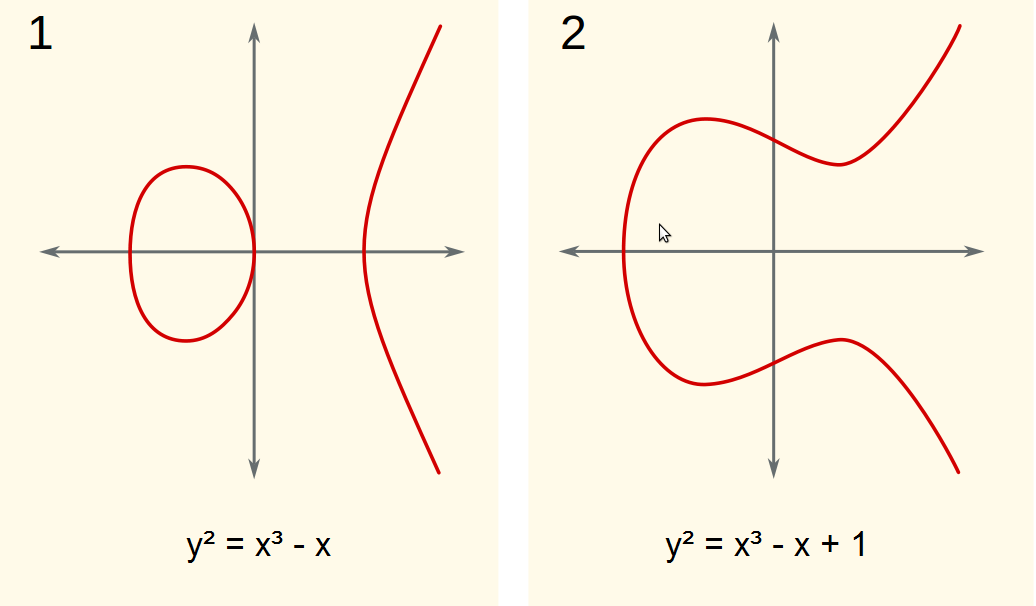
\includegraphics[scale=0.3]{EllipticCurves}\\
\caption{Courbes elliptiques sur $\RR$ }
\label{fig:ellcurve} 
Source : 
\href{http://en.wikipedia.org/wiki/Elliptic_curve}{wikipedia.org} 
\end{center}
\end{figure}


Un invariant important des courbes elliptiques s'appelle le \emph{$j$-invariant}
de $E$ :
\begin{equation}
j(E) = -1728\dfrac{(4a)^3}{\Delta}.
\end{equation}
On écrira simplement $j$ quand il n'y aura pas de confusion possible. Les deux
résultats suivant sont particulièrement intéressants :
\begin{prop}
\label{prop:j-invariant}
\begin{enumerate}[(i)]
    \item Deux courbes elliptiques définie sur un corps algébriquement clos 
        sont isomorphes si et seulement si elles ont le même $j$-invariant.
    \item Soit $j_0\in\overline{K}$ alors il existe une courbe elliptique
    $E/K(j_0)$ telle que $j(E) = j_0$.
\end{enumerate}
\end{prop}
\begin{proof}
Voir \cite[p. 45, prop. 1.4]{Sil}.
\end{proof}
On note $E/K$ pour signifier que les coefficients $a, b$ sont dans $K$, c'est
équivalent à dire que $E$ est définie sur $K$. On parle de points rationnels 
pour un corps $L\subset K$ comme les points
$P := (x,y)$ dans $E$ tel que $x, y$ sont dans $L$ et on note leur ensemble
$E(L)$.\par
\vspace{0.3cm}
Si on munit $E$ de la loi de composition de \emph{corde tangente}, désignée par
$\oplus$, alors $E$ possède une structure de groupe abélien avec pour élément 
neutre $\EO$. On dit qu'un point $P$ est un \emph{point de torsion} s'il existe 
un $m\in\ZZ$ tel que 
\begin{equation}
[m]P = \underbrace{P\oplus\dots\oplus P}_{\textup{m fois}} = \EO.
\end{equation}
On note alors l'ensemble des points de \emph{$m$-torsion} :
\begin{equation}
E[m] = \lbrace{P\in E(\overline{K}) : [m]P = \EO}\rbrace.
\end{equation}

\begin{figure}[H]
\begin{center}
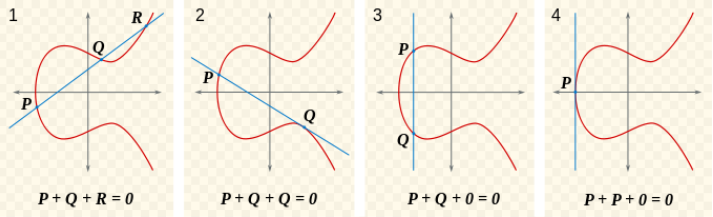
\includegraphics[width=12cm, height=3cm]{CordeTangente}
\caption{La loi corde-tangente}
\label{fig:cordetangente}
Source : 
\href{http://en.wikipedia.org/wiki/Elliptic_curve}{wikipedia.org}
\end{center}
\end{figure}

On a les résultats suivants, \emph{cf.} \cite[Cor. 6.4]{Sil}:
\vspace{0.3cm}
\begin{enumerate}[(i)]
\item Si $\textup{car}(K) = 0$ ou $\textup{car}(K) = p > 0$ et $p\nmid\,m$ 
alors :
\begin{equation}
E[m] = \zmodn{m}\times\zmodn{m}
\end{equation}
\item Si $\textup{car}(K) = p > 0$ alors on a l'une des deux situations :
    \begin{align} 
    E[p^e] &= \lbrace{\EO}\rbrace, \quad \forall
e\in\NN\setminus\lbrace{0}\rbrace\label{eq:supersingcurv}\\
    E[p^e] &= \zmodn{p^e}\quad \forall e\in\NN\setminus\lbrace{0}\rbrace
    \end{align}
\end{enumerate}
\vspace{0.3cm}

Si une courbe vérifie (\ref{eq:supersingcurv}), on dit qu'elle est
\emph{supersingulière}. On appelle \emph{$m$-ième polynôme de division} le
polynôme qui annule les abscisse d'un points de $m$-torsion.\par
Soient $E_1$ et $E_2$ deux courbes elliptiques, une \emph{isogénie} est un
morphisme \cite[p.12]{Sil} de $\varphi : E_1 \rightarrow E_2$ tel que 
$\varphi(\EO) = \EO$. C'est en fait un homomorphisme de groupe et on note 
$\textup{Hom}(E_1, E_2)$ l'ensemble des isogénies de $E_1$ vers $E_2$. 
L'ensemble $\textup{End}(E)$ des endormorphismes de $E$ est un anneau de 
caractéristique $0$, intègre et de rang au plus $4$ en tant que $\ZZ$-module. 
L'objet qui nous intéressera plus particulièrement est l'ensemble des 
endomorphismes inversibles, qu'on note $\textup{Aut}(E)$. Le théorème suivant 
détaille sa structure.
\begin{thm}
\label{th:autell}
Soit $E/K$ une courbe elliptique, alors $\textup{Aut}(E)$ est un groupe fini
d'ordre divisant $24$. Plus précisément, on a le tableau suivant :

\begin{table}[H]
\centering
\begin{tabular}{|c|c|c|}
    \hline
    \#Aut$(E)$ & $j(E)$ & car$(K)$\\
    \hline\hline
    $2$ & $j(E)\neq0,1728$ & $-$\\
    \hline
    $4$ & $j(E) = 1728$ & car$(K)\neq 2, 3$\\
    \hline
    $6$ & $j(E) = 0$ & car$(K)\neq 2, 3$\\
    \hline
    $12$ & $j(E) = 0 = 1728$ & car$(K) = 3$\\
    \hline
    $24$ & $j(E) = 0 = 1728$ & car$(K) = 2$\\
    \hline
\end{tabular}
\caption{Automorphisme de $E$ sur $\overline{K}$}
\label{tab:autoclotell}
\end{table}
\end{thm}
Les automorphismes pour les courbes elliptiques de la forme
(\ref{eq:weiersimpl}) sont tous définis par : 
\begin{equation}
x = u^2x'\etmath y = u^3y',
\end{equation}
pour $u\in\overline{K}^{\times}$; ce sont les seuls changements de variables qui
conservent cette forme.\par
Si deux courbes elliptiques $E/K$ et $E'/K$ ont le même $j$-invariant $j_0\neq0,
1728$, alors elles sont isomorphes dans une clôture algbérique de $K$, mais la 
question est de savoir sur quel corps exactement. Dans le cas où $u$ est un 
non-résidu quadratique de $K$, alors les courbes :
\begin{equation}
E : y^2 = x^3 + ax + b \etmath E^u : y^2 = x^3 + u^2ax + u^3b
\end{equation}
sont isomorphes dans $K(u)/K$ mais pas dans $K$. Dans ce cas, on dit que $E^u$
est une \emph{tordue} quadratique de $E$ sur $K$.\par
Pour les cas $j_0 = 0$ ou $1728$, on définit de façon analogue les tordues
sextiques et quarties si $u$ n'est pas un carré, ni une puissance de $3$ dans le
premier cas et s'il n'est pas un résidu quadratique à nouveau dans le second.
\subsection{Courbes elliptiques sur les corps finis}
\label{sec:curvff}
%TODO: Nombres de points, théorème de Hasse, Frobenius, trace, points de 
%torsions
On considère les courbes elliptiques sur les corps finis. Dans ce cas, une 
courbe elliptique $E/\GF{q}$ n'a qu'un nombre fini de point. Avant de donner un
résultat plus précis, on décrit un endomorphisme particulier des courbes 
elliptiques sur les corps finis.\par
Le morphisme de Frobenius $\phi_q$ agit sur les coordonnées des points de
$E(\overline{\mathbb{F}}_q)$ :
\begin{equation}
\phi_q(x,y) = (x^q, y^q)\etmath \phi_q(\EO) = (\EO),
\end{equation}
il s'agit d'un endomorphisme de $E$ et on le notera $\phi_{q,E}$. 
En particulier, on a complètement caractérisé les points rationnels d'une courbe
sur les corps finis :
\begin{equation}
P\in E(\GF{q}) \Leftrightarrow \phi_{q,E}(P) = P.
\end{equation}
\begin{prop}
Soit $E/\GF{q}$ une courbe elliptique, si on pose $t = q + 1 - \#E(\GF{q})$
alors on a :
\begin{equation}
\label{eq:frpolmin}
\phi_{q,E}^2 - t\phi_{q,E} + q = 0,
\end{equation}
en tant qu'endomorphisme de $E$ et $t$ est l'unique entier tel que l'égalité
soit vérifiée.
\end{prop}
On définit le $t$ de la proposition comme la trace du Frobenius $\phi_{q,E}$. 
En particulier, le polynôme (\ref{eq:frpolmin}) est le polynôme caractéristique 
du Frobenius de $E$, \emph{cf.} \cite[Chap. V, th. 2.3.1]{Sil}. Par abus de 
langage, on parlera parfois de $t$ comme de la trace de $E$.\par
On peut alors énoncer le résultat suivant :
\begin{thm}[Hasse]
\label{th:hasse}
Soit $E/\GF{q}$ une courbe elliptique défini sur $\GF{q}$ alors on a l'inégalité
suivante :
\begin{equation}
\vert{q + 1 - \#E(\GF{q})}\vert\leq 2\sqrt{q}.
\end{equation}
\end{thm}
\begin{proof}
\cite[Chap. V, th. 1.1]{Sil}
\end{proof}

\vspace{0.3cm}
Le groupe des $\GF{q}$-automorphismes d'une courbe elliptique sur un corps fini 
vérifie la proposition suivante :
\begin{prop}
\label{prop:autff}
Soit $E/\GF{q}$ une courbe elliptique et soit $j_0$ son $j$-invariant. Le groupe
des $\GF{q}$-automorphismes de $E$ est d'ordre :
\begin{enumerate}[(a)]
    \item $24$ si $j_0 = 0$ et $q = 4\bmod{6}$,
    \item $12$ si $j_0 = 0$ et $q = 9\bmod{12}$,
    \item $6$ si $j_0 = 0$ et $q = 1\bmod{6}$,
    \item $4$ si $j_0 = 1728$ et $q = 1, 5\bmod{12}$,
    \item $2$ dans tous les autres cas.
\end{enumerate}
\end{prop}
On a vu dans la sous-section \ref{sec:elldef} que chaque courbe a une tordue
quadratique si $j\neq0,1728$ et des tordues quartiques ou sextiques selon si $j$
est égal à $1728$ ou $0$ respectivement. Dans le cas des corps finis, on peut
même relier la trace du Frobenius de ces tordues. Les deux derniers points sont
issus d'une communication personnelle avec Luca De Feo.
\begin{prop}
\label{prop:trtwist}
Soit $E/\GF{q}$ une courbe elliptique de $j$-invariant 
$j_0\in\overline{\mathbb{F}}_q$. Si $E$ est supersingulière, alors sa trace et
celles de ses tordues sont nulles.\par
Si $E$ est ordinaire et si on note $t_E$ la trace de son Frobenius, on est dans
une des situations suivantes :
\begin{enumerate}[(i)]
\item Si $j_0\neq 0, 1728$ et si $u$ est un non-résidu quadratique de
$\GF{q}$, alors $E^u/\GF{q}$ la tordue quadratique de $E$ a pour trace :
\begin{equation}
t_{E^u} = -t_E.
\end{equation}

\item Si $j_0 = 1728$ et si $u$ est un non-résidu quadratique de
$\GF{q}$, alors $E^u/\GF{q}$ une tordue quartique de $E$ a pour trace :
\begin{equation}
t_{E^u} = \zeta_4t_{E},
\end{equation}
où $\zeta_4$ une racine \nroot{4} de l'unité de $\GF{q}$.\par

\item Si $j_0 = 0$ et $u$ n'est ni un carré, ni un cube de $\GF{q}$, alors  
$E_0^u$ une tordues sextique a pour trace :
\begin{equation}
t_{E^u} = \zeta_6t_{E_0}
\end{equation}
pour $\zeta_6$ une racine \nroot{6} de l'unité de $\GF{q}$.
\end{enumerate}
\end{prop}

\section{Complexité et notations}
Cette courte section nous permettra de définir quelques notions de complexité
et surtout d'introduire les notations qu'on utilisera pour les futures analyses
de complexité des algorithmes étudiés. Rappelons les deux définitions de base :

\begin{defn}
Soient $f$ et $g$ deux fonctions, on a $f\in O(g)$ si et seulement s'il existe 
une constante $M>0$ telle que :
\begin{equation}
    \vert{f(x)}\vert \leq M\vert{g(x)}\vert,\quad x\to\infty.
\end{equation}
On a aussi $f\in o(g)$ si et seulement si pour tout $\epsilon>0$ il existe une 
constante $N$ telle que :
\begin{equation}
    \vert{f(n)}\vert\leq\epsilon\vert{g(n)}\vert,\quad\forall n\geq N.
\end{equation}
Si en plus $g(x)$ ne s'annule pas, alors c'est équivalent à :
\begin{equation}
    \lim_{x\to\infty}{\frac{f(x)}{g(x)}} = 0.
\end{equation}
\end{defn}

On exprimera la complexité de nos algorithmes en nombre d'opérations sur 
$\GF{q}$. On note $\M{n}$ le nombre d'opérations qu'il faut pour multiplier deux
polynômes de degré au plus $n$ sur $\GF{q}$. On suppose qu'elle a les propriétés
suivantes :
\begin{equation}
\label{eq:M1}
\M{n}/n\geq\M{m}/m\textup{ si }n\geq m,\quad \M{mn} \leq m^2\M{n},
\end{equation}
pour tout $n, m\in\NN$. En particulier, elle est \emph{superlinéaire}, 
\emph{cf.} \cite{GaGe} :
\begin{equation}
\M{mn}\geq m.\M{n},\quad \M{n + m}\geq\M{n} + \M{m}, \quad \M{n}\geq n.
\end{equation}
La seconde propriété de (\ref{eq:M1}) implique que M est au plus quadratique et 
donc pour toute constante positive $c$ on a $\M{cn}\in O(\M{n})$.\par
Le nombre d'opérations nécessaires pour effectuer une multiplication dans
$\GF{q^n}$ sera noté $\E{n}\in O(\M{n})$, elle est aussi superlinéaire. De même,
on note $\I{n}$ le nombre d'opérations pour inverser un élément dans $\GF{q^n}$,
on suppose que cela prend $O(\M{n}\,\textup{log\,}n)$ opérations sur $\GF{q}$,
voir \cite{GaGe}.
On utilisera aussi la notation $\tO$, avec $f(n)\in\tO{g(n)}$
équivalent à $f(n)\in O(g(n)\,\textup{log}^k\,g(n))$.
\begin{defn}
On désignera par $\textup{rand}(F)$, la fonction retournant un élément choisi
uniformément au hasard dans un ensemble fini $F$.
\end{defn}
Le tableau suivant regroupe les différentes complexités d'opérations courantes 
sur les corps finis et leurs extensions; elles sont toutes prouvées dans 
\cite{GaGe} :
\begin{table}[H]
\centering
\begin{tabular}{|p{7cm}|c|}
    \hline
    Opération & Complexité\\
    \hline\hline
    Multiplication de deux éléments d'un anneau résiduel de degré $n$. & 
    $\E{n}$\\
    \hline
    Inversion d'un élément d'un anneau résiduel de degré $n$. &
    $O(\E{n}\,\textup{log }n)$\\
    \hline
    Exponentiation à la puissance $m$ d'un élément d'un anneau résiduel de degré
    $n$. & $O(\E{n}\,\textup{log }m)$\\
    \hline
\end{tabular}
\caption{Complexités usuelles dans $\GF{q^n}$}
\label{tab:compl}
\end{table}
\newpage
\part{Isomorphisme de corps finis}
\label{deux}
D'après le théorème \ref{th:isomGF}, deux corps finis de même cardinal sont
isomorphes. Le théorème \ref{th:elemprim} assure que toute extension de corps 
fini s'obtient par adjonction d'une racine d'un polynôme irréductible. Il y
a donc autant de façons de définir une extension que de polynômes 
irréductibles de bon degré. Le problème est comment passer d'une représentation
à l'autre.\par
%TODO Retravailler peut-être cette partie pour la rendre plus compréhensible
Soient $f$ et $g$ deux polynômes irréductibles de degré $n$ sur $\GF{q}$, on
pose :
\begin{equation}
k_1 := \GF{q}[X]/(f) \etmath k_2 := \GF{q}[Y]/(g). 
\end{equation}
On veut trouver un isomorphisme qui relie ces deux corps. Une première approche 
naïve est de chercher une racine de $f$ dans $k_2$ et d'envoyer $x = \bar{X}$ 
sur cette même racine. Cependant, cela implique de factoriser $f$, d'après 
\cite[th. 14.14]{GaGe}, factoriser complètement un polynôme de degré $n$ sur 
$\GF{q}$ prend $O(n\,\M{n}\,\textup{log}(qn))$ ou $\tO{n^2\,\textup{log\,}q}$
opérations sur $\GF{q}$. Et d'après \cite[cor. 14.16]{GaGe}, trouver une racine 
se fait en $O(M(n)\,\textup{log\;}n\textup{log}(qn))$ ou 
$\tO{n\,\textup{log\,}q}$ opérations sur $\GF{q}$. Sachant qu'on cherche une 
racine sur une extension de degré $n$, la complexité devient 
$O(\E{n}\,\textup{log\;}n\,\textup{log}(nq^n))$ ou $\tO{n^2\,\textup{log\,}q}$.
% = O~(n^3) ?
Un premier pas vers une méthode plus performante que la méthode naïve est la 
méthode de Pinch, nous allons exposer une de ses variantes dans la section 
suivante.

\section{Algorithme de Pinch}
\label{sec:algpinch}
La méthode de Pinch consiste à choisir un groupe $\Gamma$ défini par des 
relations algébriques sur $\GF{q}$ et un élément $\gamma\in\Gamma$ tel que:
\vspace{0.3cm}
\begin{enumerate}[1.]
\item il soit d'ordre $m$ petit et défini sur $\GF{q^n}$,
\item il engendre exactement $\GF{q^n}$; et non un de ses sous-corps.
\end{enumerate}
\vspace{0.3cm}
On exprime alors $\gamma$ en tant que polynôme en $x := \overline{X}$ et en 
polynôme en $y := \overline{Y}$ et on utilise ces deux expressions pour exprimer
$x$ en fonction de $y$ afin d'obtenir l'isomorphisme voulu.\par
\begin{defn}
    Soit $K/k$ et $L/k$ deux extensions de corps de degrés finis, on dit que 
    $\alpha\in K$ est \emph{relié à} $\beta\in L$ s'il existe un
    $\theta\in\textup{Hom}_k(K, L)$ tel que :
    \begin{equation}
        \theta(\alpha) = \beta.
    \end{equation}
    On dit que deux éléments $\alpha\in K$ et $\beta\in L$ sont \emph{reliés}
    ou \emph{reliés entre eux} si $\theta$ est un isomorphisme :
    \begin{equation}
        \theta : k(\alpha)\to k(\beta).
    \end{equation}
\end{defn}
En particulier, les deux expressions de $\gamma$ ont le même polynôme minimal
sur $\GF{q}$, ils sont donc reliés.
\begin{rem}
La notion est très proche de la notion d'éléments conjugués dans le sens où deux
éléments sont reliés s'ils ont le même polynôme minimal sur $k$, la 
seule différence est de niveau formel.\par
En toute généralité, $k_1$ et $k_2$ sont une même entité, le corps à $q^n$ 
éléments. Lorsqu'on descend d'un niveau d'abstraction et qu'on construit
concrètement un corps fini, on obtient des représentations différentes. Dans
ce cas, $k_1$ et $k_2$ sont deux objets distincts et par conséquent 
l'isomorphisme qui les relie n'est pas un automorphisme. On peut donc
faire une différence entre être reliés et être conjugés, bien qu'en pratique les
deux notions sont équivalentes.
\end{rem}

\subsection{Méthode cyclotomique}
Pour la méthode cyclotomique on utilisera pour $\Gamma$ le groupe multiplicatif 
de $k_1$ et $\gamma$ sera une racine primitive \nroot{m} de l'unité qui engendre
le corps $\GF{q^n}$ sur $\GF{q}$.\par
Un corps fini contient toutes les racines $m$-ièmes de l'unité si et seulement 
si l'ordre de son groupe multiplicatif est divisible par $m$. En particulier, il
contient alors des racines \nroot{m} primitives de l'unité. Soit $\zeta_m$ une
racine \nroot{m} primitive de l'unité dans $k_1$, alors l'image de $\zeta_m$ par
n'importe quel morphisme $\theta : k_1 \to k_2$ est une racine \nroot{m} 
primitive de l'unité.\par
On choisit $\zeta'_m$ une racine primitive \nroot{m} de l'unité dans $k_2$
alors $\zeta_m$ s'enverra sur une puissance de $\zeta'_m$ puisque le groupe 
mulitplicatif d'un corps fini est cyclique. On définit pour $0 < s < m$ les
applications $\theta^s : k_1 \to k_2$ , telles que :
\begin{equation}
\theta^s(\zeta_m) = (\zeta'_m)^s.
\end{equation}
Le but est de déterminer quel $\theta^s$ définit un isomorphisme ou autrement
dit de trouver deux racines de l'unité reliées entre elles.\par
Pour cela, on utilise de l'algèbre linéaire. Si on a deux bases 
$(e_i)_{i\in I}$, $(f_i)_{i\in I}$ de $k_1$, $k_2$ respectivement avec $I =
\lbrace{1,\dots,n}\rbrace$, telles qu'il existe un isomorphisme $\theta$ qui 
envoie $e_i$ sur $f_i$, alors il nous suffit de calculer la matrice de passage 
de la base $(e_i)_{i\in I}$ à $(f_i)_{i\in I}$ pour pouvoir déterminer ensuite 
$\theta(x)$. En posant $A$ la matrice avec pour lignes les $e_i$, $B$ la matrice
avec pour ligne les $f_i$ et $C$ la matrice de passage, il faut alors résoudre 
le système 
\begin{equation}
AC = B.
\end{equation}
\par
Il faut maintenant déterminer les bases $(e_i)_{i\in I}$ et $(f_i)_{i\in I}$. 
Or, les racines $m$-ièmes de l'unité engendrent l'extension, on pose alors 
$e_i = \zeta_m^i$ et $f_i = (\zeta'_m)^{si}$ selon l'application $\theta^s$ 
qu'on souhaite tester. Alors, si $\theta^s(x)$ est racine de $f$ sur $k_2$, 
l'application $\theta^s$ est effectivement un isomorphisme. La méthode peut se 
résumer ainsi :
\vspace{0.3cm}
\begin{enumerate}[1.]
    \item Trouver un entier $m$ "petit" tel que $\#\groupgen{q} = n$. 

    \item Déterminer une racine \nroot{m} primitive $\zeta_m$ dans $k_1$ et
    $\zeta'_m$ dans $k_2$.

    \item  Déterminer pour quel $s\in \lbrace{1,\dots,m-1}\rbrace$, 
    l'application $\theta^s$ telle que $\theta^s(\zeta_m) = (\zeta'_m)^s$, est 
	un isomorphisme.
\end{enumerate}
\vspace{0.3cm}
La première condition assure qu'une racine primitive \nroot{m} de l'unité 
engendre exactement $\GF{q^n}$, théorème \ref{th:polycycldecomp}. Pour le 
deuxième point, il suffit de prendre au hasard un $z\in k_1^{\times}$ et de 
l'élever à la puissance $(q^n - 1)/m$ jusqu'à tomber sur un élément d'ordre $m$,
la probabilité que cela arrive est de $\varphi(m)/m$; il y a $m$ éléments 
solution de $X^m - 1$ dans $\GF{q^n}$ et seulement $\varphi(m)$ éléments 
d'ordre exactement $m$.
\begin{ex}
Illustrons la méthode par un exemple directement tiré de l'article de 
Pinch \cite{Pin}. On considère les deux polynômes irréductibles sur $\GF{11}$, 
$f = X^{23} + 8X^2 + X + 9$ et $g = Y^{23} + 3Y^2 + 4Y + 9$. On pose $m = 829$, 
on vérifiera qu'il divise bien $11^{23} - 1$ et qu'il est premier avec $11$; 
en fait, il est lui-même premier. On définit $k_1$ et $k_2$ comme les corps de 
rupture de $f$ et $g$ respectivement.\par
Dans cet exemple, il se trouve que $\alpha(x) := x^{\tfrac{11^{23} - 1}{829}}$ 
et $\beta(y) := y^{\tfrac{11^{23} - 1}{829}}$ sont déjà des racines primitives
$829$-ième de l'unité, voici leurs expressions dans les bases monomiales 
engendrées par $x$ et $y$ :
\begin{align*}
\alpha(x) =&\hspace{0.15cm} 7 + 8x + 4x^2 + 4x^4 + 4x^5 + 10x^6 + 4x^7 + 3x^8 + 
5x^9\\
& + 2x^{10} + 6x^{11} + 4x^{12} + 8x^{13} + 6x^{14} + 4x^{15} + 4x^{16}\\
& + 5x^{17}  + 7x^{18} + 4x^{19} + x^{20} + 8x^{22},
\end{align*}
\begin{align*}
\beta(y) =&\hspace{0.15cm}1 + y + 4y^2 + 4y^3 + 9y^4 + y^5 + 6y^6 + 3y^7 + 3y^8 
+ 3y^9\\
& + 6y^{10} + 5y^{11} + 6y^{12} + 8y^{13} + y^{14} + 9y^{15} + 4y^{16}\\
& + 3y^{17} + 5y^{18} + y^{19} + 10y^{20} + 10y^{21} + 6y^{22}
\end{align*}
Le but est de calculer les matrices de passage entre les bases
$(\alpha(x)^i)_{i\in I}$ et $(\beta(y)^{si})_{i\in I}$, pour $s < 829$.
Dans ce cas précis, il se trouve que la puissance $s = 14$ convient. En 
calculant la matrice de passage, on trouve alors les coefficients de l'image de 
$x$ dans $k_2$ sur la deuxième ligne de la matrice de passage et l'image de $x$ 
est :
\begin{align*}
\theta(x) =&\hspace{0.15cm} 8 + 9y + y^2 + 2y^3 + 7y^4 + 4y^5 + 6y^6 + 10y^7 + 
9y^8\\
& + 10y^9 + 2y^{10} + 2y^{12} + 10y^{13} + 2y^{14} + 7y^{15} + y^{16}\\
& + 3y^{17} + 2y^{18} + 2y^{20} + y^{21} + y^{22}
\end{align*}
On peut alors vérifier que $f(\theta(x)) = 0$.
\end{ex}

\subsection{Limitations}
Le premier problème de cette méthode est qu'il n'y a pas toujours d'élément
d'ordre "petit" dans $\GF{q^n}^{\times}$. Par exemple, si on prend $p = 2$ et un
un entier $k$ tel que $n = 2^k - 1$ soit premier, on ne trouvera pas d'élement 
d'ordre plus petit que $2^n - 1$. Il y a donc un risque qu'on soit obligé de 
chercher des éléments d'ordre proche de $q^n - 1$, on obtiendrait alors une 
complexité exponentielle en $n$.\par
Un autre problème est la recherche au hasard des racines primitives de l'unité. 
Le côté aléatoire du choix fait qu'il n'est jamais certain de pouvoir tomber sur
deux racines qui sont dans le même facteur irréductible du polynôme
cyclotomique. Il peut arriver qu'on soit obligé de tester jusqu'à $O(m)$ valeurs
différentes de $s$ pour pouvoir enfin tomber sur un isomorphisme.\par
Le problème vient du fait suivant. Il se trouve que dans un corps fini $\GF{q}$
si la classe de $q$ n'engendre pas $\zmodninv{m}$ alors le polynôme cyclotomique
$\Phi_m$ se scinde en $e := \varphi(m)/n$ facteurs irréductibles distincts de 
degré $n$ dans $\GF{q}[X]$ où $n := \ord{m}{q}$, \emph{cf.} 
\ref{th:polycycldecomp}. Autrement dit :
\begin{equation}
\Phi_m(X) = P_1(X)\dots P_e(X)\in\GF{q}[X],
\end{equation}
avec $\textup{deg}(P_i) = n$. Lorsqu'on choisit deux racines de l'unité au
hasard, il est donc possible qu'elles ne soient pas racines du même facteur
irréductible. C'est pour cela qu'il faut \og{parcourir}\fg{} les racines de
l'unité afin d'espérer tomber sur deux racines ayant le même polynôme minimal
dans $\GF{q}[X]$, c-à-d. trouver deux racines qui ont la même orbite sous
l'action du groupe de Galois.\par
Ces deux problèmes sont résolus par l'algorithme de Rains traité dans la section
suivante.
\section{Algorithme de Rains : méthode cyclotomique}
La méthode de Rains cyclotomique est une extension de la méthode de Pinch
cyclotomique. Les principaux changements sont l'utilisation de petites
extensions des corps considérés afin de pouvoir trouver un $m$ plus petit et
l'usage des \emph{périodes de Gauss} afin de déterminer des éléments étant dans 
la même orbite sous l'action du groupe de Galois de l'extension.

\subsection{Principe}

L'algorithme se résume de la façon suivante. On commence par chercher un $m$ qui
satisfait certaines conditions permettant de trouver des racines $m$-ièmes
primitives de l'unité qui engendrent les corps qui nous intéressent.\par
Si on ne trouve pas de $m$ assez petit, il se peut qu'on ait besoin de
travailler dans de petites extensions de $k_1$ et $k_2$, voir
\ref{sec:extension}. Il faut alors construire des élements reliés de $k_1$ et 
$k_2$ ou de leurs extensions, ce qui est effectué \textit{via} les 
\emph{périodes de Gauss} dans la section \ref{sec:gaussper}.\par
Si l'utilisation d'une extension a été nécessaire, alors on calcule la trace des
deux éléments obtenus afin d'avoir des générateurs de l'extension qui nous
intéresse. Une fois ceux-ci obtenus, il ne reste plus qu'à déterminer
l'isomorphisme, ce qui est traité dans la section \ref{sec:elemnorm}.

\subsection{Utilisation d'une extension}
\label{sec:extension}
La première limitation de la méthode de Pinch est la taille du facteur
$m$, Rains propose \cite{Rai} alors  de passer par une petite
extension de $\GF{q^n}$ afin de trouver un $m$ plus petit. En effet, imaginons 
qu'on ait deux extensions de petit degré $k'_1$ et $k'_2$ de $k_1$ et $k_2$ 
respectivement. Si on applique la méthode de Pinch à $k'_1$ et $k'_2$ et 
qu'on trouve un isomorphisme, il suffira alors de le restreindre à $k_1$.\par
L'idée est la suivante, soient $o$ et $m$ deux entiers tels que $q$ soit d'ordre
$n.o$ dans $\zmodninv{m}$. Soient maintenant $k_1'/k_1$ et $k_2'/k_2$ deux
extensions de degré $o$, d'après la section précédente, on peut trouver deux
racines de l'unité $\zeta_m\in k_1'$ et $\zeta'_m\in k_2'$ reliées qui 
engendrent $k_1'$ et $k_2'$ en tant qu'extensions de $\GF{q}$. Si on note
$\theta$ l'isomorphisme qui relie $\zeta_m$ à $\zeta'_m$ alors on a : 
\begin{equation}
\theta(\textup{Tr\;}_{k'_1/k_1}(\zeta_{m})) =
\textup{Tr\;}_{k'_2/k_2}(\zeta'_{m}).
\end{equation}
La surjectivité de la trace, \cite[Chap. VI, th. 2.5]{Lan1}, permet d'assurer en
particulier que ces éléments engendrent toujours $k_1$ et $k_2$. On résume la 
situation par le schéma suivant :

\begin{equation}
\begin{tikzpicture}
\matrix(m)[matrix of math nodes,
row sep=0.5em, column sep=1.5em,
text height=2ex, text depth=1ex]
{\GF{q}[\zeta_m]& & \\
&\GF{q}[\Tr{\zeta_m}]&\\
\GF{q^o}& & \\
&\GF{q}& \\};
\path[-,font=\scriptsize,>=angle 90]
(m-1-1) edge node[below] {$o$} (m-2-2)
(m-3-1) edge node[below] {$o$} (m-4-2)
(m-1-1) edge node[left] {$n$} (m-3-1)
(m-2-2) edge node[left] {$n$} (m-4-2);
\end{tikzpicture}
\end{equation}

Le problème de devoir tester plusieurs candidats avant de tomber sur un 
isomorphisme est malheureusement toujours présent. Pour pallier à ce problème,
on utilise alors les périodes de Gauss introduites à la section  
\ref{sec:gaussper}.


\subsection{Périodes de Gauss}
\label{sec:gaussper}
On souhaite obtenir deux éléments reliés afin de pouvoir en déduire
l'image de $x$ \emph{via} la méthode décrite dans la section \ref{sec:elemnorm}.
On rappelle que deux éléments sont reliés s'ils définissent un isomorphisme ou
de manière équivalente s'ils ont le même polynôme minimal. Pour cela, on va 
sommer suffisamment de racines primitives $m$-ièmes de l'unité pour obtenir des
éléments qui ont la même orbite sous l'action du groupe de Galois.\par
Soit $K$ un corps de nombres et $\EO_K$ son anneau des entiers. Posons 
$\mathfrak{p}$ l'idéal de $\EO_K$ au-dessus de $p$ tel que $\EO_K/\mathfrak{p} =
\GF{q}$, pour $q = p^r$. Si on pose $K[\mu_m]/K := K[X]/\Phi(X)$ où $\mu_m := 
\mu_{m,\overline{\CC}}$ alors on a le schéma suivant :
\begin{equation}
\label{schema:gaussnorm}
\begin{tikzpicture}
\matrix(m)[matrix of math nodes,
row sep=1em, column sep=3em,
text height=1.5ex, text depth=0.25ex]
{ &K[\mu_m] & \GF{q}[\mu_m] & \\
\QQ[\mu_m]& & &\GF{p}[\mu_m]\\
& K & \GF{q}& \\
\QQ& & &\GF{p}\\};
\path[-,font=\scriptsize,>=angle 90]
(m-2-1) edge node[left] {$\zmodninv{m}$} (m-4-1)
(m-3-2) edge node[left] {$G$} (m-1-2)
(m-1-3) edge node[right] {$\groupgen{q}$} (m-3-3)
(m-4-4) edge node[right] {$\groupgen{p}$} (m-2-4)
(m-2-1) edge node[auto] {} (m-1-2)
(m-4-1) edge node[auto] {} (m-3-2)
(m-1-3) edge node[auto] {} (m-2-4)
(m-3-3) edge node[auto] {} (m-4-4);
\path[->>,font=\scriptsize,>=angle 90]
(m-4-1) edge node[auto] {$\bmod p$} (m-4-4)
(m-3-2) edge node[auto] {$\bmod\mathfrak{q}$} (m-3-3)
(m-1-2) edge node[auto] {$\bmod\mathfrak{Q}$} (m-1-3);
\end{tikzpicture}
\end{equation}
Où $\zmodninv{m}$ est le groupe de Galois de $\QQ[\mu_m]/\QQ$, $G$ est le groupe
de Galois de $K[\mu_m]/K$, sous-groupe de $\zmodninv{m}$ et $\groupgen{q}$
le groupe de décomposition de 
$\mathfrak{Q}/\mathfrak{q}$, %($= \GF{q}[\mu_m]/\GF{q}$ ?)
on a en particulier l'inclusion $\groupgen{q}\subset G
\subset\zmodninv{m}$.

%%%%%%%%%%%%%%%%%%%%%%%%%%%%%%%%%%%%%%%%%%%%%%%%%%%%%%%%%%%%%%%%%%%%%%%%%%%%%%%%
\iffalse
\begin{equation}
\#G/\groupgen{q}=g\etmath\#\groupgen{q} = f = [K[\mu_m]:K]/g.
\end{equation}
\fi
%%%%%%%%%%%%%%%%%%%%%%%%%%%%%%%%%%%%%%%%%%%%%%%%%%%%%%%%%%%%%%%%%%%%%%%%%%%%%%%%
%TODO: Rajouter ce qui reste ? À voir ce dont on a besoin pour la
%démonstration...

\begin{defn}
Supposons qu'il existe un sous-groupe $S\subset\zmodninv{m}$ tel que
$\zmodninv{m} = \groupgen{q}\times S$. Pour toute racine \nroot{m} de
l'unité $\zeta_m$ dans $\GF{q^n}$, on définit la \emph{période de Gauss} 
$\eta(\zeta_m)$
comme suit :
\begin{equation}
\eta(\zeta_m) = \sum_{\sigma\in S}{\zeta_m^{\sigma}}.
\end{equation}
\end{defn}
\begin{prop}
\label{prop:gaussperconj}
Le groupe de Galois $\textup{Gal}(\GF{q}[\mu_m]/\GF{q})\simeq\groupgen{q}$
agit transitivement sur les périodes de Gauss $\eta(\zeta_m)$ pour tout
$\zeta_m\in\mu_m^{\times}$.
\end{prop}
\begin{proof}
Soit $\tau\in\groupgen{q}$, alors :
\begin{equation}
\eta(\zeta_m)^{\tau} = \sum_{\sigma\in S}{\zeta_m^{\sigma\tau}}
\end{equation}
comme $\zmodninv{m} = \groupgen{q}\times S$ alors tous les générateurs
$\zeta'_m$ de $\mu_m$ apparaissent à droite, d'où $\groupgen{q}$ agit 
transitivement sur les $\eta(\zeta_m)$.
\end{proof}
\begin{rem}
En particulier, en tant qu'éléments de $\GF{q^n}$ les $\eta(\zeta_m)$ sont
conjugués. Ainsi, quand on les considère sous deux représentations différentes,
elles sont reliées entre elles.
\end{rem}
Le but de la section est de démontrer le théorème suivant :

\begin{thm}
\label{th:gausspernorm}
Soit $\GF{q^n}/\GF{q}$ une extension de degré $n$ et soit un entier $m$ premier 
avec $q$, tel que :
\vspace{0.3cm}
\begin{enumerate}[(i)]
    \item $\zmodninv{m} = \groupgen{q}\times S$ pour $S$ un sous-groupe de
        $\zmodninv{m}$,
	\item $\#\groupgen{q} = n$
    \item $(\varphi(m), r) = 1$,
    \item $m$ est sans facteur carré.
\end{enumerate}
\vspace{0.3cm}
Alors les périodes $\eta(\zeta_m)$ forment une base
normale de $\GF{q^n}$ sur $\GF{q}$.
\end{thm}

La condition (iii) implique que $\groupgen{p} = \groupgen{q}$ et donc que
$\eta(\zeta_m)$ engendre $\GF{q}[\mu_m]/\GF{q}$ si et seulement s'il engendre
$\GF{p}[\mu_m]/\GF{p}$. Cela permet d'éviter des discussions supplémentaires 
lors de la preuve, on se contentera donc de traiter le cas $q = p$.\par
Pour démontrer le théorème, on va remonter en caractéristique zéro pour
finalement retomber sur le résultat qu'on souhaite obtenir. On a l'anneau 
\begin{equation}
\EO_{m,p} := \GF{p}[X]/\Phi_m(X),
\end{equation}
réduction modulo $\mathfrak{p}$ de 
\begin{equation}
\EO_m := \ZZ[X]/\Phi_m(X),
\end{equation}
l'anneau des entiers de $\QQ[X]/\Phi_m(X)$ d'après le théorème 
\ref{th:entiercycl} et $\mathfrak{p} = p\EO_m$ est l'idéal de $\EO_m$ au-dessus 
de $p$. Comme $\QQ[X]/\Phi_m(X)$ est galoisienne, proposition 
\ref{prop:cyclgal}, de groupe de Galois $\zmodninv{m}$, alors il agit sur 
$\EO_m$ et donc sur $\EO_{m,p}$.\par
Soit maintenant $S$ un sous-groupe de $\zmodninv{m}$, on va étudier la forme de 
l'invariant $\EO_{m,p}^S$  de $\EO_{m,p}$ sous l'action de $S$, réduction modulo
$\mathfrak{p}$ de $\EO_m^S$ l'invariant de $\EO_m$ sous l'action de $S$.\par
On a $\mathfrak{p} = \prod_{i=0}^g{\mathfrak{P}_i}$, où $g$ est le nombre
d'idéaux de $\EO_m$ au-dessus de $p$ et les $\mathfrak{P}_i$ sont des premiers
de $\EO_m$. En effet, l'extension est galoisienne et $p$ est non ramifié dans 
$\EO_m$ puisque $m$ et $p$ sont premiers entre eux, théorème 
\ref{th:entiercycl}. Ainsi on a :
\begin{equation}
\EO_{m,p} = \EO_m/p\EO_m = \EO_m/\prod_{i=0}^g{\mathfrak{P}_i}
\end{equation}
D'après le théorème des restes chinois généralisé, on obtient finalement :
\begin{equation}
\EO_{m,p} = \prod_{i=0}^g{\EO_m/\mathfrak{P}_i}
\end{equation}
Or, les $\EO_m/\mathfrak{P}_i$ sont des extensions de corps de $\ZZ/p\ZZ\simeq
\GF{p}$ de même degré, le degré résiduel $f = [\EO_m/\mathfrak{P}_i:\GF{p}]$. 
Dans ce cas, on a :
\begin{equation}
\label{eq:structinvSmodp}
\EO_{m,p}^S = \prod_{i=0}^{g'}{\GF{p^{f'}}}.
\end{equation}
où $g'$ est le nombre d'idéaux $\mathfrak{P}'_i$ de $\EO_m^S$ tels que $p\EO_m^S
= \prod_{i = 0}^{g'}{\mathfrak{P}'_i}$ et $f' = 
[\EO_m^S/\mathfrak{P}'_i:\GF{p}]$.

\begin{lem}[Rains \cite{Rai}]
\label{lem:nbprimeabove}
Soit $p$ un nombre premier tel que $(m, p) = 1$ et soit $S$ un sous-groupe de
$\zmodninv{m}$. Alors le nombre d'idéaux premiers de $\EO_m^S$ au-dessus de $p$ 
est l'indice du sous-groupe engendré par $p$ dans $\zmodninv{m}/S$.
\end{lem}
\begin{proof}
Commençons par le cas $S = \groupgen{1}$, alors d'après l'identité fondamentale,
on a $\varphi(m) = gf$, $g$ et $f$ définis comme ci-dessus. En prenant en compte
le fait que le corps résiduel $\EO_m/p\EO_m$ est un corps fini, l'action du 
groupe de Galois est uniquement constitué d'éléments de la forme $p^k$.
Mais cela implique que le degré du corps résiduel est donc l'ordre de $p$ dans 
$\zmodninv{m}$ ce qui donne le résultat pour $S = \groupgen{1}$ car dans ce cas 
:
\begin{equation}
g = \varphi(m)/f = [\zmodninv{m}:\groupgen{p}].
\end{equation}

Considérons maintenant le cas d'un sous-groupe $S$ quelconque, comme 
$\QQ[\mu_m]/\QQ$ est abélienne alors $\QQ[\mu_m]^S/\QQ$ est aussi galoisienne 
de groupe de Galois $\zmodninv{m}/S$. Alors on peut reporter l'étude à 
l'extension $\QQ[\mu_m]^S/\QQ$, on regarde l'action de $\zmodninv{m}/S$ sur les
$\mathfrak{P}'_i$ tels que $p\EO_m^S = \prod_{i=0}^{g'}{\mathfrak{P}'_i}$. Comme
il n'y a qu'une seule orbite de cardinal $g'$ alors la formule des classes
donne :
\begin{equation}
g' = \frac{\#\zmodninv{m}/S}{\#\groupgen{p}} = 
[\zmodninv{m}/S:\groupgen{p}].
\end{equation}
\end{proof}

\begin{cor}[Rains \cite{Rai}]
L'anneau $\EO_{m,p}^S$ se factorise en une somme directe de
$[\zmodninv{m}/S:\groupgen{p}]$ corps tous isomorphes à $\GF{p^n}$, où $n$ est 
l'ordre de $p$ dans $\zmodninv{m}/S$.
\end{cor}
\begin{proof}
Il suffit d'appliquer le lemme \ref{lem:nbprimeabove}, l'équation
(\ref{eq:structinvSmodp}) et le fait que $\groupgen{p}$ étant le groupe
décomposition de $\mathfrak{p}$, son cardinal $\#\groupgen{p}$ est égal à 
$e'f'$, où $e'$ est l'indice de ramification de $\mathfrak{p}$ dans $\EO_m^S$, 
qui est égal à $1$, et $f'$ le degré du corps résiduel, qui est égal à $n$.
\end{proof}
En particulier si $[\zmodninv{m}/S:\groupgen{p}] = 1$ alors $\EO_{m,p}^S$ est
un corps; c'est en fait exactement $\GF{p^n}$, avec $\#\groupgen{p} = n$. Il 
reste alors à montrer que les périodes de Gauss engendrent effectivement 
$\EO_{m,p}^S$.
\begin{lem}[Rains \cite{Rai}]
Soit $m$ un entier sans facteur carré, alors les périodes $\eta(\zeta_m^k)$
engendrent $\EO_{m,p}^S$, où $k\in\zmodninv{m}/S$.
\end{lem}
\begin{proof}

Commençons par considérer le cas $S = \langle1\rangle$ et $m$ premier. Alors on 
a $\eta(\zeta_m^k) = \zeta_m^k$ et, par définition, les $\zeta_m^k$ engendrent 
$\EO_{m,p}$ pour $0 \leq k\leq m$. Il suffit alors de montrer que $1$ peut 
s'exprimer en fonction des $\zeta_m^k$ pour $k > 0$, puisque $k = 0$ n'est pas 
dans $\zmodninv{m}$. Mais $m$ est premier, alors le polynôme $\Phi_m$ 
donne exactement :
\begin{equation}
\textup{Tr}(\zeta_m) = \sum_{0 < k < m}{\zeta_m^k} = 1.
\end{equation}

Changeons alors seulement l'hypothèse $m$ premier en $m$ sans facteur carré, on 
va raisonner par récurrence. En particulier, on peut écrire $m = m_1m_2$ avec 
$(m_1,m_2) = 1$ et le résutlat ci-dessus est encore valable pour $m_1$ et 
$m_2$. D'après le théorème des restes chinois, on a :
\[\zmodninv{m} \simeq \zmodninv{m_1} \times \zmodninv{m_2},\]
ainsi, \textit{via} cet isomorphisme on peut exprimer un élément
$\eta(\zeta_m^k)$ de $\EO_{m,p}$ comme un produit de deux éléments
$\eta(\zeta_m^{k_1})$ et $\eta(\zeta_m^{k_2})$ dans $\EO_{m_1,p}$ et 
$\EO_{m_2,p}$, avec $k_1\in\zmodninv{m_1}$ et $k_2\in\zmodninv{m_2}$ 
respectivement, et inversement.
%TODO: C'est vraiment utile tout ce qui suit ?
%%%%%%%%%%%%%%%%%%%%%%%%%%%%%%%%%%%%%%%%%%%%%%%%%%%%%%%%%%%%%%%%%%%%%%%%%%%%%%%%
\iffalse
En effet, prenons un $k\in\zmodninv{m}$ alors on peut l'écrire sous la forme :
\[k = uk_2m_1 + vk_1m_2\]
avec $k_1\in\zmodninv{m_1}$, $k_2\in\zmodninv{m_2}$ et $u,v\in\mathbb{Z}$ tels 
qu'ils soient premiers avec $m_2$ et $m_1$ respectivement. On a donc :
\begin{align*}
z_S^{(k)} &= \zeta_m^k\\
&= \zeta_m^{uk_2m_1 + vk_1m_2}\\
&= (\zeta_m^{um_1})^{k_1}(\zeta_m^{vm_2})^{k_2}\\
\end{align*}
On a bien que $\zeta_m^{um_1}$ est une racine \nroot{$m_2$} puisque 
$m_1m_2 = m$, mais c'est aussi une racine primitive car $(u,m_2) = 1$ et 
$(m_1, m_2) = 1$; donc la seul façon d'avoir $kum_1 = m$ est de poser $k = m_2$.
Le raisonnement est exactement le même pour l'autre terme. D'où le résultat :
\[z_S^{(k)} = z_S^{(k_1)}z_S^{(k_2)}\].\par
Pour l'autre sens, on prend le produit suivant :
\[z_S^{(k_1)}z_S^{(k_2)} = \zeta_{m_1}^{k_1}\zeta_{m_2}^{k_2}\]
Si on l'élève à la puissance $m_1$ ou $m_2$, le produit ne pourra pas être égal 
à $1$. En revanche, si on l'élève à la puissance $m$, on obtiendra bien $1$, 
d'où le fait que c'est une racine primitive \nroot{m} de l'unité. Alors on 
pourra toujours le réécrire sous la forme : 
\[\zeta_m^k = z_S^{(k)}\]
avec $k\in\zmodninv{m}$, ce qu'on cherchait.\par
\fi
%%%%%%%%%%%%%%%%%%%%%%%%%%%%%%%%%%%%%%%%%%%%%%%%%%%%%%%%%%%%%%%%%%%%%%%%%%%%%%%%
Ainsi, comme les $\eta(\zeta_m^{k_1})$ engendrent $\EO_{m_1,p}$ et les 
$\eta(\zeta_m^{k_2})$ engendrent $\EO_{m_2,p}$ par réccurence, alors les 
$\eta(\zeta_m^k)$ engendrent $\EO_{m,p}$, à nouveau par le théorème des restes 
chinois.\par
Pour finir, on considère $S$ un sous-groupe quelconque du groupe de Galois. 
Prenons un $\alpha$ dans $\EO_{m,p}^S$, alors on peut écrire :
\begin{equation}
\alpha = \sum_{\sigma\in S}{\beta^{\sigma}}
\end{equation}
pour un $\beta$ dans $\EO_{m,p}$; l'action d'un $\sigma$ sur $\alpha$ ne sera 
alors qu'une permutation des termes de la somme. De plus, on peut aussi écrire 
$\beta$ sous la forme :
\begin{equation}
\beta = \sum_{k\in\zmodninv{m}}{c_{k}\zeta_m^{k}}
\end{equation}
c'est ce qu'on a prouvé plus haut. En combinant les deux expressions on obtient 
alors :
\begin{align*}
\alpha &= \sum_{\sigma\in
S}{\sum_{k\in\zmodninv{m}}{c_{k}\zeta_m^{k\sigma}}}\\
&= \sum_{k\in\zmodninv{m}/S}{c_k\eta(\zeta_m)^{k}}\\
\end{align*}
ce qu'il fallait démontrer.
\end{proof}

Ainsi, si $\zmodninv{m}/S = \groupgen{p}$ et $\#\groupgen{p} = n$, alors si $m$ 
est sans facteurs carrés, les $\eta(\zeta_m^k)$ avec $k\in\groupgen{p}$ 
engendrent $\GF{p^n}$ d'après le lemme précédent, la condition (ii) implique que
ce sont aussi des générateurs de $\GF{q^n}$ et la proposition 
\ref{prop:gaussperconj} implique qu'ils sont conjugués. Ceci achève la preuve du
théorème \ref{th:gausspernorm}.

\subsection{Éléments normaux}
\label{sec:elemnorm}
Imaginons qu'on ait calculé deux éléments normaux $v\in k_1$ 
et $w\in k_2$ reliés, c-à-d. tels que $\theta(v) = w$. Pour finir de résoudre le
problème, il faut déterminer les images $\theta(x^i)$ pour $0\leq i < n$. Or, 
comme $\theta(x^i) = \theta(x)^i$, il suffit de déterminer uniquement la valeur 
de $\theta(x)$.\par
Pour cela, il faut pouvoir être capable de déterminer les coefficients de $x$
dans la base engendré par un élément normal $v$ :
\begin{equation}
\label{eq:elemnorm1}
x = \sum_{i\in I}{c_iv^{q^i}}
\end{equation}
alors on aura :
\begin{align}
\theta(x) &= \sum_{i\in I}{c_i\theta(v)^{q^i}}\label{eq:elemnorm2}\\
&= \sum_{i\in I}{c_iw^{q^i}}\label{eq:elemnorm3}
\end{align}
puisque $\theta$ est un morphisme. Devoir passer de la base normale à la base 
monomiale en $x$ peut se faire, non pas en inversant une matrice, comme cela a
été fait en \ref{sec:algpinch} mais en inversant l'élément d'un anneau quotient.
C'est ce qui va être exposé dans cette sous-section. 
Dans le cas des corps finis, on a montré que le Frobenius engendre le groupe de 
Galois de $\GF{p^n}$, donc pour un $x\in\GF{p^n}$ ses conjugués sont 
$x^p, x^{p^2},\dots,x^{p^{n-1}}$. 
Le corollaire du théorème suivant permet d'utiliser des éléments normaux 
dans le cadre de l'utilisation d'une extension comme cela a été expliqué à la
sous-section précédente.
\begin{thm}
\label{th:nbelemnorm}
Le nombre d'élements normaux dans $\GF{p^n}$ est égal au nombre d'unités de
l'anneau $\GF{p}[X]/(X^n - 1)$.\par
\end{thm}
\begin{proof}
Voir \cite[th. 3.73]{LiNi2}.
\end{proof}
\begin{cor}[Rains \cite{Rai}]
\label{cor:tracenorm}
Soit $L/K$ une extension de corps finis de caractéristique $p$, premier. Si
$x\in L$ est un élément normal de $L$ sur $K$, alors $\textup{Tr}_{L/K}(x)$ est 
un élément normal de $K$ sur $\GF{p}$. Si de plus$[L:K]$ est une puissance de 
$p$ alors la réciproque est aussi vraie.
\end{cor}
\begin{proof}
Puisque la trace est surjective sur les corps finis, alors pour tout $y\in K$ il
existe un $y'\in L$ tel que $y = \textup{Tr}_{L/K}(y')$. Il suffit alors 
de prendre l'expression de $y'$ dans la base normale engendrée par $x$ et d'y 
appliquer la trace; le fait qu'elle soit linéaire montre que 
$\textup{Tr}_{L/K}(x)$ est aussi une base normale de $K$.\par
Montrons l'autre sens. Supposons que $K = \GF{q}$ et $L = \GF{q^{p^k}}$ où $q
= p^n$. D'après le théorème \ref{th:nbelemnorm}, le nombre d'éléments normaux de
$L$ est égal au nombre d'unité dans $\GF{p}[X]/(X^{p^kn} - 1)$. Comme
$(X^{p^kn} - 1 ) = (X^n - 1)^{p^k}$, alors un élément de $\GF{p}[X]/(X^{p^kn} - 
1)$ est une unité si et seulement si sa réduction modulo $(X^n - 1)$ est une
unité dans $\GF{p}[X]/(X^n - 1)$.
Comme dans ce cas, $(X^n - 1)^{p^k} \subset (X^n - 1)$, on a $\GF{p}[X]/
(X^n - 1) \subset \GF{p}[X]/(X^{p^kn} - 1)$, une unité du premier anneau sera 
donc une unité du second; et comme la réduction de $1$ modulo quoique ce soit 
est toujours $1$, une unité de $\GF{p}[X]/(X^n - 1)$ est nécessairement une 
unité de $\GF{p}[X]/(X^{p^kn} - 1)$.\par
On en déduit que $L$ a $p^k$ fois plus d'éléments normaux que $K$. De façon plus
générale, un élément de $K$ a exactement $p^k$ antécédents pour la trace, le
nombre de conjugués, puisque l'extension est galoisienne; donc $L$ a au plus
$p^k$ fois élément normaux que $L$. La borne est atteinte dans notre cas, ce qui
conclut la démonstration.
\end{proof}

Comme expliqué plus haut, on veut trouver les coefficients de $x$ dans la base 
normale engendrée par $v$, en déduire son image dans la base normale engendrée 
par $w$ et pour finir son image dans la base monomiale engendrée par $y$. Si on 
pose $I := \lbrace{0,\dots,n-1}\rbrace$, la situation se 
résume par le schéma suivant :
\begin{equation}
\begin{tikzpicture}
\matrix(m)[matrix of math nodes,
row sep=3em, column sep=5em,
text height=2ex, text depth=2ex]
{\bigoplus\limits_{i\in I}{\GF{q}\cdot x^i} & \bigoplus\limits_{i\in
I}{\GF{q}\cdot y^i}\\
\bigoplus\limits_{i\in I}{\GF{q}\cdot v^{p^i}} & \bigoplus\limits_{i\in
I}{\GF{q}\cdot w^{p^i}}\\};
\path[->,font=\scriptsize,>=angle 90]
(m-1-1) edge node[auto] {} (m-1-2)
(m-2-1) edge node[auto] {$\phi$} (m-2-2)
(m-1-1) edge node[left] {$\pi$} (m-2-1)
(m-2-2) edge node[right] {$\pi^{\prime}$} (m-1-2);
\end{tikzpicture}
\end{equation}

L'application $\GF{q}$-linéaire $\pi^{\prime}$ est donnée par l'expression de 
$w$ en fonction des $y^i$ ceci équivaut à l'évaluation d'un polynôme en une
variable et prend $O(n^2)$ opérations, voir \cite[th. 5.1]{GaGe}. La seule 
application qui pose un problème est celle correspondant à $\pi$ qui permet 
d'exprimer $x$ en fonction des $v^{p^i}$. C'est pour cette application qu'on va 
devoir effectuer tout le travail. Soit $z\in\GF{q^n}$ alors il existe des 
$c_i\in\GF{q}$ tels que :
\begin{equation}
z = \sum_{0 \leq i < n}{c_iv^{q^i}}.
\end{equation}
En appliquant $\phi_{q^{n-j}}$ puis une forme $\GF{q}$-linéaire $\lambda
: \GF{q^n} \to \GF{q}$ dont on précisera la nature plus loin, on obtient :
\begin{equation}
\lambda\left(z^{q^{n-j}}\right) = \sum_{0\leq i < n}
{c_i\lambda\left(v^{q^{i+n-j}}\right)}.
\end{equation}
Soit maintenant la matrice $B = (b_{ij})_{(i,j)\in I^2}$ définie par :
\begin{equation}
b_{ij} = \lambda\left(v^{q^{i+n-j}}\right).
\end{equation}
Si la matrice est inversible alors on a terminé, puisque si on note $d_{ij}$ les
coefficients de $B^{-1}$, on a bien :
\begin{equation}
c_i = \sum_{0\leq j < n}{d_{ij}\lambda\left(z^{q^{n-j}}\right)},
\end{equation}
pour $0\leq i < n$. Reste à savoir si la matrice $B$ sera effectivement 
inversible.\par
D'après un résultat classique d'algèbre linéaire, toute forme linéaire peut
s'exprimer sous la forme :
\begin{equation}
x \mapsto \Tr{\alpha x},
\end{equation}
pour un certain $\alpha\in\GF{q}$. On peut donc réécrire les coefficients de $B$
sous la forme suivante :
\begin{equation}
b_{ij} = \Tr{\alpha v^{q^{i+n-j}}} = \Tr{\alpha^{q^j}v^{q^i}}.
\end{equation}
On va voir que dans notre cas, il nous suffira de choisir $\alpha = v$.

\begin{lem}[Rains \cite{Rai}]
\label{lem:mattrinv}
Soit $\alpha,\beta\in\GF{q^n}$ et soit la matrice $A$ définie par les 
coefficients $a_{ij} = \Tr{\alpha^{q^i}\beta^{q^j}}$, $A$ est inversible si et 
seulement si $\alpha$ et $\beta$ sont des éléments normaux.
\end{lem}
\begin{proof}
Supposons que $\alpha$ ne soit pas un élément normal. Dans ce cas, il existe une
relation de dépendance linéaire entre les conjugués de $\alpha$, alors la 
combinaison linéaire des lignes de $A$ correspondant à cette dépendance est $0$
puisque la trace est linéaire; $A$ ne peut donc pas être inversible.\par
Inversement, supposons que $A$ ne soit pas inversible. Il existe alors une 
combinaison linéaire de ses lignes qui vaut $0$. Ou encore, il existe une 
combinaison linéaire $\alpha^{\prime}$ des conjugués $\alpha$ telle que 
$\Tr{\alpha^{\prime}\beta^{q^j}} = 0$ pour tout $j$ entre $0$ et $n-1$; 
c-à-d. telle que :
\[\Tr{\alpha^{\prime}\beta + \alpha^{\prime}\beta^q + \dots + 
\alpha^{\prime}\beta^{q^{n-1}}}\]
Or la trace est surjective, donc si $\beta$ est normal cela implique que 
$\alpha^{\prime} = 0$ mais alors $\alpha$ n'est pas un élément normal; ce qui 
démontre le lemme.
\end{proof}
Il se trouve que la matrice $B$ a une propriété particulière, 
elle est ce qu'on appelle une matrice \emph{circulante}, c-à-d. si :
\[i_1 - j_1 \equiv i_2 - j_2 \bmod n\]
alors on a 
\[b_{i_1j_1} = b_{i_2j_2}\]
et inversement. Donc, si on considère :
\[b_{i+1j+1} = \lambda\left(v^{q^{(i+1) + n - (j+1)}}\right) = 
\lambda\left(v^{q^{i+n-j}}\right)\]
on a bien que $b_{ij} = b_{i+1j+1}$ avec $(i+1) - (j+1) \equiv i - j \bmod n$ 
comme annoncé plus haut. On a alors le théorème suivant :

\begin{thm}
\label{th:matcirciso}
Les matrices circulantes de $M_n(\GF{q})$ forment un anneau qui est isomorphe à 
$\mathbb{F}_q[\omega]/(\omega^n - 1)$ \textup{via} l'isomorphisme suivant :
\begin{equation*}
\label{eq:isomconvert}
\psi : B \longmapsto \sum_{0\leq j < n}{b_{0j}\omega^j}.
\end{equation*}
\end{thm}
\begin{proof}
Montrons que l'application $\psi$ est un morphisme d'anneaux. On a bien 
évidemment $\psi(I_n) = 1$ et de manière relativement immédiate :
\begin{align*}
\psi(A + B) &= \sum_{0\leq j < n}{(a_{0j} + b_{0j})\omega^j}\\
&= \sum_{0\leq j < n}{a_{0j}\omega^j} + \sum_{0\leq j < n}{b_{0j}\omega^j}\\
&= \psi(A) + \psi(B).
\end{align*}
Maintenant, d'après la formule du produit de deux polynômes, on a :
\begin{align*}
\psi(A)\psi(B) &= \sum_{0\leq k < n}
{\bigg(\sum_{i+j=k}{a_{0i}b_{0j}}\bigg)\omega^k}\\
&= \sum_{0\leq k < n}{\bigg(\sum_{i\equiv k-j \bmod n}{a_{0i}b_{0(k-i \bmod n)}}
\bigg)\omega^k}.
\end{align*}
Mais $b_{0k-i} = b_{ik}$ puisque $0 -(k-i) \equiv i-k \bmod n$; en tenant compte
du fait que $i$ parcourt tout $\zmodn{n}$, on arrive finalement à :
\[\sum_{0\leq k < n}{\bigg(\sum_{0\leq i < n}{a_{0i}b_{ik}}\bigg)\omega^k} = 
\psi(AB).\]\par
Comme les $\omega^k$ sont linéairement indépendants par définition, pour que 
l'image d'une matrice circulante soit égale à $0$, il faut que sa première 
ligne, et donc toutes les autres, soit nulle; d'où $\textup{Ker}\,\psi = 
\{0_n\}$. La surjectivité est immédiate, il suffit de prendre les coefficients 
d'un élément quelconque $u$ de $\GF{q}[\omega]/(\omega^n - 1)$ et de définir la 
matrice $A$ de coefficients $a_{ij} = u_{(i-j \bmod n)}$ pour $i,j\in\zmodn{n}$,
où les $u_i$ sont les coefficients $u$; on aura alors $\psi(A) = u$.
\end{proof}
En résumé, si on pose $z = x$, on a :
\[\textup{Tr}\left(x^{p^{n-j}}\right) = \sum_{0\leq i < n}{c_i\textup{Tr}
\left(v^{p^{i+n-j}}\right)}\]
et la matrice $B$ est définie par :
\[b_{ij} = \Tr{\alpha v^{p^{i+n-j}}} = \Tr{\alpha^{p^j}v^{p^i}}\]
On sait qu'elle est inversible grâce au lemme \ref{lem:mattrinv}, donc si on
note $d_{ij}$ les coefficients de la matrice $B^{-1}$, on a bien :
\[c_i = \sum_{0\leq j < n}{d_{ij}\textup{Tr}\left(x^{p^{n-j}}\right)}\]
Le théorème \ref{th:matcirciso} et les formules (\ref{eq:elemnorm1}),
(\ref{eq:elemnorm2}) et (\ref{eq:elemnorm3}) permettent de conclure.
\subsection{Algorithme et analyse de complexité}
\label{sec:algcompcycl}
Maintenant qu'on a tous les résultats théoriques qu'il nous faut, on va pouvoir
énoncer et justifier les algorithmes pour déterminer l'isomorphisme. 
On rappelle brièvement la situation, on a $f$ et $g$ deux polynômes 
irréductibles de degré $n$ distincts sur $\GF{q}$, on note :
\[k_1 := \GF{q}[X]/(f)\etmath k_2 := \GF{q}[Y]/(g)\]
avec $q = p^r$ pour $r$ un entier naturel non nul, $p$ un nombre premier
impair et $r$ premier avec $n$. Il nous faut alors déterminer deux éléments 
reliés et en déduire l'image de $x := \overline{X}$ pour déterminer complètement
l'isomorphisme. 

\subsubsection*{Calcul de générateurs reliés}
Comme cela a été exposé au point \ref{sec:extension}, si on ne trouve pas de $m$
assez petit alors il faut passer par une extension de petit degré $o$ de
$\GF{q^n}$ afin de pouvoir appliquer les résultats à l'extension $\GF{q^{n.o}}$
et redescendre sur $\GF{q^n}$.\par
La façon dont on va trouver $m$ est détaillée dans la section
\ref{sec:recherchemcycl}. En résumé, on cherche le plus petit entier
$m$ sans facteurs carrés tel qu'il existe $o\in\NN\setminus\lbrace{0}\rbrace$ 
satisfaisant :
\vspace{0.3cm}
\begin{enumerate}[(i)]
    \item $(q, m) = 1$ et $q$ est d'ordre $\ord{m}{q} :=n.o$ dans 
    $\zmodninv{m}$,
    \item $\varphi(m)/n$ et $n$ sont premiers entre eux,
    \item $n$ et $o$ sont premiers entre eux,
    \item $(\varphi(m), r) = 1$ pour $q = p^r$,
    %\item $\zmodninv{m} = \groupgen{q^o}\times S$ pour $S$ un sous groupe
    %de $\zmodninv{m}$ d'ordre $\varphi(m)/(n.o)$.
\end{enumerate}
\vspace{0.3cm}
Les conditions $(i)$ et $(ii)$ assurent que les racines $m$-ièmes de l'unité
engendrent exactement $\GF{q^{n.o}}$ (\emph{cf.} 
\ref{schema:gaussnorm}); elles impliquent aussi que $\zmodninv{m} =
\groupgen{q^o}\times S$ pour $S$ un sous-groupe d'ordre $\varphi(m)/(n.o)$, ce
qui permet d'appliquer le théorème \ref{th:gausspernorm}. La condition $(3)$ est
d'ordre pratique et permet de construire des extensions à partir de polynôme à 
coefficients directement dans $\GF{q}$ si besoin est. La condition permet $(iv)$
d'assurer que $\groupgen{p} = \groupgen{q}$ et donc que les résultats sur
$\GF{p}$ soient encore valables sur $\GF{q}$.
\begin{rem}
La condition $(iv)$ implique que $(r,n) = 1$ et cette condition ne peut pas être
affaiblie à $(r,n)\neq1$. En effet, on a $\groupgen{q}\times S = \zmodninv{m}$, 
donc par définition $p = sq^a\bmod m$ pour un $s\in S$ et $0 \leq a < n$, alors 
$q=s^rq^{ar} \bmod m$. Or, $q$ ne peut être écrit que d'une seule façon comme 
produit d'un élément de $S$ et d'une puissance de $q$, d'où $s^r = 1$ et $q^{ar 
- 1} = 1 \bmod m$. Ce qui implique que $n$ divise $ar - 1$ et donc que $(n, r) =
1$.\par
Une solution possible serait de calculer un générateur $\alpha$ de 
$k/\GF{p^{d/c}}$, son polynôme minimal serait alors uniquement défini sur 
$\GF{p^{d/c}}$ mais se scinderait en $c$ facteurs sur $\GF{q}$, ce qui nous 
obligerait à réutiliser la méthode trial-and-error de Pinch. Une autre solution
serait d'utiliser la méthode elliptique qu'on va décrire à la section
\ref{sec:algell}.
\end{rem}
\vspace{0.3cm}
Ainsi selon la valeur de $o$ lorsqu'on cherche $m$, c-à-d. si $o = 
\ord{m}{q} /n = 1$ ou $> 1$, il y aura deux façons de procéder, c'est ce qu'on 
va détailler plus bas.
\paragraph{$\bullet$ Cas rationnel $o = 1$}
Imaginons qu'on ait trouvé un $m$ satisfaisant les conditions $(i)$ à $(iv)$ 
avec $o = 1$. Dans ce cas, on peut travailler directement dans les corps $k_1$ 
et $k_2$ pour calculer les périodes de Gauss. Le tout est résumé dans 
l'algorithme \ref{alg:gausspersansext}.

\begin{algorithm}
\caption{Calcul d'une période de Gauss}
\label{alg:gausspersansext}
\begin{algorithmic}[1]
\REQUIRE $k$ une extension de degré $n$; $m$ un entier divisible par $n$
satisfaisant les conditions $(i)$ à $(iv)$; $\mathcal{M}$ ensemble des diviseurs
stricts de $m$.
\ENSURE $\eta$ un élément normal de $k$ reliés aux autres périodes de Gauss.
\bigskip
\REPEAT
    \STATE $\zeta_m \leftarrow \textup{rand}(k)^{(q^n - 1)/m}$
\UNTIL{$\zeta_m^m = 1\quad\&\quad\forall 
    d\in\mathcal{M},\,\zeta_m^d\neq1$}
\STATE $\eta \leftarrow \sum_{a\in S}{\zeta_m^a}$
\RETURN $\eta$
\end{algorithmic}
\end{algorithm}
On veut déterminer sa complexité, pour trouver une racine primitive 
\nroot{m} de l'unité, on prend un élément au hasard dans $\GF{q^n}$, on l'élève 
à la puissance $(q^n - 1)/m$ et on teste si le résultat élevé à la puissance 
$m/\ell$ vaut $1$ ou non pour $\ell$ un diviseur premier strict de $m$. On 
s'attend à ce que cela réussisse après $O(1)$ essais; chaque essai prenant 
\begin{equation}
O(\E{n}n\,\textup{log\;}q)
\end{equation}
opérations.\par
On doit ensuite calculer la période de Gauss $\eta := \eta(\zeta_m)$,
d'après ce qui précède cela revient à faire $\varphi(m)/n$ exponentiation dans
$\GF{q^n}$ d'exposant au plus $m$, cela se fait en 
\begin{equation}
O((m\textup{log\;}m)\E{n}/n) 
\end{equation}
opérations.\par
Ainsi, le coût total de l'algorithme est de 
\begin{equation}
O(\E{n}(n\,\textup{log\;}q + m\,\textup{log\;}m/n))
\end{equation}
opérations dans $\GF{q}$. Tant que $m\in o(n^2)$, on 
peut négliger les termes en $m$ et on obtient la proposition suivante :
\begin{prop}
\label{prop:algsansext}
L'algorithme \ref{alg:gausspersansext} est correct et de complexité
\begin{equation}
O(\E{n}n\,\textup{log\,}q).
\end{equation}
\end{prop}

\paragraph{$\bullet$ Cas général $o > 1$}
Si jamais $q$ n'est pas d'ordre $n$ alors on doit passer par une extension de
degré $o = \ord{m}{q}/n$ premier avec $n$; si $(o,n)\neq1$ on passe au
$m$ suivant (\emph{cf.} \ref{sec:recherchemcycl}). Pour cela on définit $h$ dans
$\GF{q}[X]$, irréductible de degré $o$ et on définit les extensions :
\begin{equation}
k_1' := k_1[U]/(h) \etmath k_2' := k_2[V]/(h)
\end{equation}
dans lesquelles on travaillera. Si on pose $\eta_1 = \sum_{\sigma\in
S}{\zeta_m^{\sigma}}$ et $\eta_2 = \sum_{\sigma\in S}{\zeta_m'^{\sigma}}$ alors
on peut résumer la situation au schéma suivant :
\begin{equation}
\begin{tikzpicture}
\matrix(m)[matrix of math nodes,
row sep=3em, column sep=3em,
text height=1.5ex, text depth=0.25ex]
{\GF{q}[\eta_1] & \GF{q}[\eta_2]\\
\GF{q}[\Tr{\eta_1}] & \GF{q}[\Tr{\eta_2}]\\};
\path[->,font=\scriptsize,>=angle 90]
(m-1-1) edge node[auto] {} (m-1-2)
(m-2-1) edge node[auto] {$\theta$} (m-2-2);
\path[-,font=\scriptsize,>=angle 90]
(m-1-1) edge node[left] {$o$} (m-2-1)
(m-1-2) edge node[right] {$o$} (m-2-2);
\end{tikzpicture}
\end{equation}

\vspace{0.3cm}
\begin{algorithm}
\caption{Calcul d'une période de Gauss \emph{via} une extension}
\label{alg:gaussperavecext}
\begin{algorithmic}[1]
\REQUIRE $k$ un corps fini de cardinal $q^n$; $m$ un entier satisfaisant les 
conditions $(i)$ à $(iv)$; $h$ un polynôme de degré $o$ à coefficients dans 
$\GF{q}$; $\mathcal{M}$ ensemble des diviseurs stricts de
$m$.
\ENSURE $\eta$, un élément normal unique de $k$ sous l'action de Galois.
\bigskip
\STATE $k' \leftarrow k/(h)$
\REPEAT
    \STATE $\zeta_m \leftarrow \textup{rand}(k')^{(q^{n.o} - 1)/m}$
\UNTIL{$\zeta_m^m = 1$\quad\&\quad$\forall 
    d\in\mathcal{M},\,\zeta_m^d\neq1$}
\STATE $\alpha \leftarrow \sum_{a\in S}{\zeta_m^a}$
\STATE $\eta \leftarrow \textup{Tr}_{k'/k}(\alpha)$
\RETURN $\eta$
\end{algorithmic}
\end{algorithm}
La procédure est décrite dans l'algorithme \ref{alg:gaussperavecext}. Le calcul 
de sa complexité est assez proche de celle de l'algorithme 
\ref{alg:gausspersansext}. La grosse différence se situe au niveau de la 
construction de l'extension de degré $no$ et dans le calcul de la trace de 
$\eta$. On suppose avoir déjà une table de polynômes irréductibles  
sur $\GF{p}$ de sorte que le calcul de $h$ est gratuit. On suppose alors 
que la construction d'une extension de $\GF{q}$ est en $O((no)^2)$ opérations 
sur $\GF{q}$. Le nombre d'opérations nécessaire à la recherche d'une racine 
primitive \nroot{m} de l'unité est, de façon analogue au cas précédent, en :
\begin{equation}
O(\E{no}\,no\,\textup{log }q)
\end{equation}
opérations sur $\GF{q}$. De même, la complexité du calcul d'une période de Gauss
sur $\GF{q^n}$ est en 
\begin{equation}
O((m\,\textup{log }m)\,\E{no}/(no)).
\end{equation}
Le calcul de la trace quant à lui peut être effectué en $O((no)^2)$ ou est en
$O(\E{no})$ opérations, dans les deux cas, il est négligeable face au reste.\par
La remarque sur la taille de $m$ est encore valable dans le cas présent. Si
$m\in O((no)^2)$, alors le pire cas possible est $no = \varphi(m)$. On en déduit
le résultat suivant.
\begin{prop} 
\label{prop:algavecext}
L'algorithme \ref{alg:gaussperavecext} calcule correctement un élément normal
$\eta$ relié aux autres périodes de Gauss en 
\begin{equation}
O(\E{no}(no)\,\textup{log }q).
\end{equation}
opérations sur $\GF{q}$.
\end{prop}
\begin{proof}
Le théorème \ref{th:gausspernorm} et la proposition \ref{prop:gaussperconj}
assurent que $\alpha$ est un élément normal unique de $\GF{q^{n.o}}$. Il suffit 
alors d'appliquer le corollaire \ref{cor:tracenorm} pour assurer que $\eta :=
\Tr{\alpha}$ soit un élément normal de $\GF{q^n}$.
\end{proof}
\begin{rem}
L'algorithme ci-dessus est au mieux quadratique en $n$. De même, la première
partie de l'algorithme est au mieux quadratique en $p$; les expériences ont
confirmé cette tendance et ont montré que la construction d'extension devient
très vite prohibitive en même temps que $o$ augmente.
\end{rem}

\subsubsection*{Changement de la base normale vers la base monomiale}
Il reste alors à déterminer exactement l'isomorphisme, c'est-à-dire calculer son
image en $x$. Comme on l'a expliqué au début de la sous-section
\ref{sec:elemnorm}, si on a deux bases normales, il suffit d'exprimer les 
coefficients de $x$ par rapport à la base normale engendrée par $\eta(\zeta_m)$;
alors il suffit de reporter les coefficients trouvés dans la base normale 
engendrée par $\eta(\zeta'_m)$. On rappelle l'existence de l'isomorphisme 
reliant les matrices circulantes de tailles $n$ sur $\GF{q}$ et l'anneau 
$\GF{q}[\omega]/(\omega^n - 1)$ vu en section \ref{sec:elemnorm}. La procédure
décrite dans cette section est résumée dans l'algorithme \ref{alg:convert}.

\begin{algorithm}
\caption{Conversion de la base monomiale vers la base normale}
\label{alg:convert}
\begin{algorithmic}[1]
\REQUIRE $z\in\GF{q^n}$, $v$ élément normal, $n$ degré de l'extension, $p$ 
caractéristique, $\omega$ défini ci-dessus.
\ENSURE $c$, tuple contenant les coefficients de $z$ dans la base 
normale engendrée par $v$.
\bigskip
\FOR{$i = 0$ \TO $n-1$}
    \STATE $B_i \leftarrow \Tr{v\times v^{q^{n-(i+1)}}}$
\ENDFOR
\STATE $I \leftarrow (\sum_{i = 0}^{n-1}{B_i\cdot \omega^i})^{-1}$
\FOR{$i = 0$ \TO $n-1$}
    \STATE $T_i \leftarrow \Tr{v\times z^{q^{n-i}}}$
\ENDFOR
\FOR{$i = 0$ \TO $n-1$}
    \STATE $c_i \leftarrow \sum_{j=0}^{n-1}{I_{(j-i)\bmod n}T_j}$
\ENDFOR
\RETURN $c$

\end{algorithmic}
\end{algorithm}
Calculons sa complexité. De la ligne $1$ à $3$, la complexité est dominée par 
l'élévation de $v$ à la puissance $q^n$, le calcul de sa trace et la somme du 
résultat $n$ fois. Cela revient à élever à la puissance $q^n$ des polynômes à 
coeffcient dans $\GF{q}$ et à la somme d'éléments de $\GF{q}$. D'où 
\begin{equation}
O(n\E{n}\,\textup{log}\;q) + n\textup{T}(n) = O(n\E{n}\,\textup{log}\;q) 
\end{equation}
opérations sur $\GF{q}$, où $\textup{T}(n)$ est la complexité du calcul de la 
trace d'un élément de $\GF{q^n}$ et $\textup{T}(n) \in O(\E{n})$ \cite[th.
7.9]{GaSho}.\par
À la ligne $4$, il s'agit dans un premier temps de la multiplication par un 
scalaire d'éléments de $\mathbb{F}_p[\omega]/(\omega^n - 1)$ puis de $n$ sommes 
de polynômes. Ensuite, on inverse le polynôme et on prend la trace de l'élément 
qu'il représente; ce qui nous donne 
\begin{equation}
O(\E{n}\,\textup{log }n)
\end{equation}
opérations sur $\GF{q}$.\par
Des lignes $5$ à $7$, il s'agit de la même opération que des lignes 1 à 3, d'où 
encore une complexité de 
\begin{equation}
O(n\E{n}\,\textup{log}\;q).
\end{equation}

Les lignes 8 à 10 consistent en $n$ sommes de $n$ multiplications dans le corps 
de base $\GF{q}$, c-à-d. $O(n)$ opérations.\par
\begin{prop}
\label{prop:algconvert}
L'algorithme \ref{alg:convert} calcule correctement les coefficients de $x$ dans
la base normale engendrée par $v$ en
\begin{equation}
O(n\E{n}\,\textup{log}\;q)
\end{equation}
opérations sur $\GF{q}$.
\end{prop}
\begin{rem}
Bien que la complexité soit la même que les deux algorithmes précédents, il se
trouve qu'en pratique cette méthode est extrêmement lente comme on le verra dans
la partie \ref{trois}.
\end{rem}

\subsubsection*{Algorithme principal}

On peut désormais énoncer complètement l'algorithme de Rains cyclotomique : on
commence par chercher le plus petit entier $m$ qui satisfait les conditions
$(1)$ à $(4)$, on calcule alors les périodes de Gauss dans $k_1$ et $k_2$ ou
dans leurs extensions et on finit par calculer les coefficients de $x$ dans la
base normale engendrée par $\eta_2$; en réécrivant $\eta_2$ en fonction de $y$,
on retrouve alors l'image de $x$ dans la base monomiale engendrée par $y$ et on
peut calculer l'image de n'importe quel élément de $k_1$. Le tout est résumé
dans l'algorithme \ref{alg:rainscycl}.
\begin{algorithm}
\caption{Calcul d'un isomorphisme de corps finis}
\label{alg:rainscycl}
\begin{algorithmic}[1]
\REQUIRE $k_1$, $k_2$ deux corps finis à $q^n$ éléments
\ENSURE $\phi(x)$ l'image de la classe de $X$ par un isomorphisme $\phi : k_1
\to k_2$. 
\bigskip
\STATE Chercher le plus petit entier $m$ satisfaisant $(1)$ à $(5)$
\STATE $o \leftarrow \ord{m}{q}/n$
\IF{$o = 1$}
    \STATE Calculer $\eta_1$ en utilisant l'algorithme \ref{alg:gausspersansext}
    \STATE Calculer $\eta_2$ en utilisant l'algorithme \ref{alg:gausspersansext}
\ELSE
    \STATE Trouver un polynôme irréductible $h$ de degré $o$ sur $\GF{q}$
    \STATE Calculer $\theta_1$ en utilisant l'algorithme 
    \ref{alg:gaussperavecext}
    \STATE Calculer $\theta_2$ en utilisant l'algorithme 
    \ref{alg:gaussperavecext}
    \STATE $\eta_1 \leftarrow \Tr{\theta_1}$
    \STATE $\eta_2 \leftarrow \Tr{\theta_2}$
\ENDIF
\STATE Construire $\GF{q}[\omega]/(\omega^n - 1)$
\STATE Calculer les $c_i$ en utilisant l'algorithme \ref{alg:convert}

\RETURN $\sum_{i\in\lbrace{0,\dots,n-1}\rbrace}{c_i\eta_2^{q^i}}$

\end{algorithmic}
\end{algorithm}

\section{Algorithme de Rains : méthode elliptique}
\label{sec:algell}
%TODO: Résumer/Détailler le papier de Luca, rajouter les résultats sur
%les twists, les périodes, détaillés l'algorithme et sa complexité, le prouver 
%(probablement fait avec le papier de Luca et Mihailescu pour les périodes ?)
%, détailler les différentes étapes, les paramètres, la façon de trouver m 
%etc.
Utiliser pour groupe algébrique $\Gamma$ le groupe des points d'une courbe
elliptique avait déjà été proposé par Pinch \cite{Pin} et également par Rains
\cite{Rai}. Cependant Rains a renoncé à la développer plus en détails, jugeant
qu'elle n'était pas prometteuse. La complexité théorique n'étant pas
foncièrement différente que celle de la méthode cyclotomique, on a voulu
développer la variante de cet algorithme et l'implanter dans le but de comparer
avec la méthode cyclotomique.\par
Comme pour la méthode cyclotomique, on cherche des points d'ordre petit $m$ 
divisant le nombre de point d'une courbe elliptique et, en utilisant les mêmes 
techniques que pour la méthode faisant usage des racines de l'unité, on essaie 
de trouver un isomorphisme reliant leurs abscisses.
\subsection{Principe}
%TODO: Choix d'un point d'ordre m sur une bonne courbe elliptique engendre 
%l'extension, utilisation des périodes elliptiques afin d'avoir un élément 
%stable par l'action du groupe de Galois (Énoncer les lemmes etc.)
On commence par chercher un entier $m$ et une courbe $E/\GF{q}$ tels que
les abscisse de points de $m$-torsion engendrent $\GF{q^n}$; ce sera
étudié plus en détail dans la section \ref{sec:choixparam}.\par
Il faut alors calculer des points d'ordre exactement $m$ sur $E/k_1$ et $E/k_2$.
De façons analogue à la méthode cyclotomique, on calcule alors ce qu'on appelle 
les \emph{périodes elliptiques} qui consistent à sommer les abscisses de 
l'orbites d'un point d'ordre $m$ sous l'action du groupe de Galois, ce sera 
détaillé dans la section \ref{sec:perell}. On aura alors obtenu deux éléments 
reliés et accessoirement normaux, il suffira alors de procéder comme dans la 
méthode cyclotomique \ref{sec:algcompcycl} afin d'obtenir l'isomorphisme désiré.

\subsection{Choix des paramètres}
\label{sec:choixparam}
%TODO: Justifier le choix de m par rapport à n et q, tout ce qui concerne la 
%valeur propre d'ordre n et donc le choix de traces qui s'en suit, expliquer 
%comment on pick les courbes (à ce moment là on pourra aussi justifier avec le 
%résultat sur les tordues).
On rappelle qu'une courbe elliptique $E/\GF{q}$ est munie de l'endomorphisme de
Frobenius $\phi_q : [X, Y, Z] \mapsto [X^q, Y^q, Z^q]$ qui a pour polynôme
minimal $X^2 -tX + q$ avec $\#E(\GF{q}) = q + 1 - t$, en particulier, le
polynôme minimal se scinde dans une extension de degré quadratique imaginaire de
$\QQ$ et on a 
\begin{equation}
t = \alpha + \beta\etmath \alpha\beta = q, 
\end{equation}
pour $\alpha,\beta\in\CC$. On rappelle aussi que 
\begin{equation}
\#E(\GF{q^n}) = q^n + 1 - (\alpha^n + \beta^n), 
\end{equation}
voir par exemple \cite[th. 2.3.1, chap V]{Sil}.\par
Si $m$ est premier avec $p$ alors le groupe de $m$-torsion $E[m]$ est de rang
$2$ et si on fixe une base de $E[m]$, alors $\phi_q$ agit sur $E[m]$ comme une 
matrice $2\times2$ à coefficients dans $\zmodn{m}$.
\begin{defn}
Soit $E/\GF{q}$ une courbe elliptique ordinaire, un nombre premier $m$ est 
appelé nombre \emph{premier d'Elkies} pour $E$ si le polynôme minimal de 
$\phi_q$ se scinde en deux facteurs distincts dans $\zmodn{m}$.
\end{defn}
\begin{rem}
Les premiers $m$ tels que le polynôme minimal de $\phi_q$ ne se scinde pas
dans $\zmodninv{m}$ sont appelés des nombres premiers de Atkin. Il se trouve que
la proportion de nombres premiers de Elkies pour une courbe elliptique donnée 
est de $1/2$, pour plus de précisions consulter \cite{Scho}.
\end{rem}
Si $m$ est un premier de Elkies, alors il existe une base de $E[m]$ sur 
laquelle $\phi_q$ agit comme une matrice diagonale :
\begin{equation}
\begin{pmatrix}
\alpha & 0\\
0 & \beta
\end{pmatrix}
\end{equation}
et pour tout entier $n$, le Frobenius de $E/\GF{q^n}$ agit comme la puissance
\nroot{n} de cette matrice sur $E[m]$. Ainsi, l'extension de degré
$k = \textup{min}(\ord{m}{\alpha},\ord{m}{\beta})$ de 
$\GF{q}$ est la plus petite extension contenant un point d'ordre $m$. En
effet, si on prend $P\in E[m]$ dans l'espace propre de $\alpha$  et que 
$\ord{m}{\alpha} = k$, alors :
\begin{equation}
\phi_{q^k}(P) = [\alpha^k]P = [1]P = P.
\end{equation}
Autrement dit, si $\ord{m}{\alpha} = n$ et $\ord{m}{\beta}$ ne divise pas $n$,
alors $\GF{q^n}$ ne contient que $m$ points d'ordre $m$. Il se trouve qu'on a pu
observer que les abscisses de ces points engendrent $\GF{q^n}$, c'est l'objet de
la conjecture \ref{conj:gaussellnorm}. Elles jouent donc un rôle analogue aux 
racines primitives $m$-ièmes de l'unité pour la méthode cyclotomique.\par

À l'instar des racines de l'unité qui ne sont pas nécessairement racines du même
polynôme minimal, les abscisses des points d'ordres $m$ ne sont pas
nécessairement racine du même facteurs du $m$-ième polynôme de division. Il
faut donc trouver un moyen de générer des points tels qu'en
sommant leurs abscisses on obtienne des éléments qui ont le même polynôme
minimal, c'est ce que vont faire les périodes elliptiques.

\subsection{Périodes elliptiques}
\label{sec:perell}
%TODO: Prouver et définir les périodes elliptiques 
La caractéristique principale de l'algorithme de Rains, comme on a pu le voir
dans la section précédente, est la détermination de deux éléments reliés
par un isomorphisme. Ici, il se trouve que l'unicité sera déduite de
l'action du Frobenius de la courbe elliptique choisie $E/\GF{q}$ sur des points
de torsion d'ordre $m$ de la courbe $E(\GF{q^n})$.\par
Si on essaie de définir les périodes elliptiques comme dans le cas des périodes
de Gauss, on rencontre un phénomène qui n'était pas présent dans le cas
précédent. Les courbes elliptiques possèdent des automorphismes non-triviaux qui
ne peuvent pas être laissés de côté. On rappelle la proposition
\ref{prop:autff}.\par
\begin{defn}
Soit $E/\GF{q}$ une courbe elliptique avec $p\neq2, 3$ et soit $m > 2$
un nombre premier de Elkies. On considère le cas 
$j(E)\notin\lbrace{0, 1728}\rbrace$ et soit $\alpha\in\zmodninv{m}$ une valeur 
propre de $\phi_q\bmod{m}$. Supposon que $\zmodninv{m}/\lbrace{\pm1}\rbrace = 
\groupgen{\alpha}\times S$ pour $S$ un sous-groupe de $\zmodninv{m}$. Alors pour
tout point $P$ de $m$-torsion dans l'espace propre de $\alpha$, on définit la 
période elliptique $\eta_{\alpha}(P)$ de la façon suivante :
\begin{equation}
\label{eq:ellperpar}
\eta_{\alpha}(P) = \sum_{\sigma\in S}{([\sigma]P)_X}
\end{equation}
où $P_X$ désigne l'abscisse du point $P$.\par
Pour $j = 0$ ou $1728$, on suppose que $\#\textup{Aut}_{\GF{q}}(E)$ divise
$\varphi(m)$ et on identifie $\textup{Aut}_{\GF{q}}(E)$ à un sous-groupe de 
$\zmodninv{m}$. On suppose à nouveau que $\zmodninv{m}/\textup{Aut}_{\GF{q}} = 
\groupgen{q}\times S$ et on peut définir les périodes elliptiques
$\eta_{\alpha}(P)$ dans ces deux cas particuliers :
\begin{equation}
\label{eq:ellpergen}
\eta_{\alpha}(P) = \sum_{\sigma\in S}
{\left([\sigma]P\right)_X^{\#\textup{Aut}_{\GF{q}}(E)/2}}
\end{equation}
On remarque en particulier que (\ref{eq:ellperpar}) n'est qu'un cas particulier
de (\ref{eq:ellpergen}) pour $\textup{Aut}_{\GF{q}}(E) = \lbrace{\pm1}\rbrace$.
\end{defn}
\begin{prop}
L'endomorphisme de Frobenius $\phi_q$ agit transitivement sur les périodes 
elliptiques $\eta_{\alpha}(P)$.
\end{prop}
\begin{proof}
Comme $P$ est dans l'espace propre de $\alpha$, lui appliquer 
$\phi_q$ revient à le multiplier par $\alpha$. Si on prend 
$\tau\in\groupgen{\alpha}$ alors on a pour $d\geq1$ tel que $\alpha^d = \tau 
\bmod m$ :
\begin{equation}
\phi_q^d(\eta_{\alpha}(P)) = \sum_{\sigma\in
S}{\left([\sigma][\tau]P\right)_X^{\#\textup{Aut}(E)/2}}
\end{equation}
Or, on a $\zmodninv{m}/\textup{Aut}(E) = \groupgen{\alpha} \times S$ donc
tous les points de l'espace propre $\alpha$ apparaissent dans la somme de
droite, ce qui conclut la preuve.
\end{proof}
On peut alors énoncer la conjecture principale :
\begin{conj}
\label{conj:gaussellnorm}
Soient $m$ un nombre premier différent de $p$ et $t$ un entier tels que :
\vspace{0.3cm}
\begin{enumerate}[1.]
    \item $|t| < \sqrt{2q}$,
    \item $X^2 - tX + q = (X - \alpha)(X - \beta)\bmod{m}$,
    \item $\zmodninv{m}/\textup{Aut}_{\GF{q}} = \groupgen{\alpha}\times S$ pour
    $S$ un sous-groupe de $\zmodninv{m}$,
    \item $\ord{m}{\alpha} = n$ et $\ord{m}{\beta}\nmid n$.
\end{enumerate}
\vspace{0.3cm}
Soit $E/\GF{q}$ une courbe elliptique de trace $t$. Dans ce cas, $\GF{q^n}$ est
la plus petite extension contenant des points d'ordre $m$ et pour tout $P$ 
d'ordre $m$ dans l'espace propre de $\alpha$, les périodes elliptiques $\eta_
{\alpha}(P)$ forment une base normale de $\GF{q^n}$ sur $\GF{q}$.\par
\end{conj}

La situation est résumée dans le schéma suivant dû à Luca De Feo, inspiré de
\cite{MiMoScho} :
\begin{center}
\begin{tikzpicture}
\matrix(m)[matrix of math nodes,
row sep=1em, column sep=2em,
text height=1ex, text depth=0.25ex]
{K(E[m]) & & \\
& K(E[m]_X) & \GF{q}(E[m]_X) \\
K(E_{\alpha}) & & \\
& K(E_{\alpha, X}) & \GF{q}(E_{\alpha, X})\\
K^{\prime} & & \\
& K = \QQ(j)[X]/\Phi_m(j,X) & \GF{q}\\
& \QQ(j) &\\};
\path[-,font=\scriptsize]
(m-7-2) edge node[auto] {$m + 1$} (m-6-2)
(m-6-2) edge node[auto] {} (m-4-2)
(m-4-2) edge node[auto] {} (m-2-2)
(m-6-3) edge node[right] {$\groupgen{\alpha}$} (m-4-3)
(m-4-3) edge node[auto] {} (m-2-3)
(m-5-1) edge node[auto] {} (m-3-1)
(m-3-1) edge node[auto] {} (m-1-1)
(m-6-2) edge node[auto] {Aut($E$)} (m-5-1)
(m-4-2) edge node[auto] {Aut($E$)} (m-3-1)
(m-2-2) edge node[auto] {Aut($E$)} (m-1-1);
\path[->>,font=\scriptsize,>=angle 90]
(m-6-2) edge node[auto] {} (m-6-3)
(m-4-2) edge node[auto] {} (m-4-3)
(m-2-2) edge node[auto] {} (m-2-3);
\end{tikzpicture}
\end{center}

\begin{rem}
Les expériences tendent évidemment à valider ce résultat et bien que la preuve 
ne soit pas clairement établie, on a de bonnes raisons de croire qu'elle est 
loin d'être inaccessible. Des pistes sont présentes dans 
les articles \cite{MiMoScho} et \cite{CouRe}, seul le manque de temps nous a
empêché de les explorer. 
\end{rem}

\subsection{Algorithme et analyse de complexité}
\label{sec:algcompell}
%TODO: Décrire l'algorithme et donner sa complexité.
La deuxième partie de l'algorithme pour trouver un isomorphisme étant déjà 
traité dans la section \ref{sec:algcompcycl}, nous allons nous concentrer sur la
recherche de deux éléments reliés, autrement dit, sur le calcul des périodes 
elliptiques.\par
On cherche donc un entier $m$ tel que $n\mid\varphi(m)$ et tel qu'il existe au 
moins un $t\in\zmodninv{m}$ satifaisant :

\vspace{0.3cm}
\begin{enumerate}[(1)]
    \item si $m$ est égal à $p$, alors :
	\begin{equation}
	\ord{m}{t} = n \etmath\zmodninv{m}/\textup{Aut}_{\GF{q}}(E) = 
	\groupgen{t}\times S
	\end{equation}
	pour $S$ sous-groupe de $\zmodninv{m}$
    \item si $m$ est un premier différent de $p$, on veut alors que :
	\begin{equation}
	X - tX + q = (X - \alpha)(X - \beta)\bmod{m}
	\end{equation}
	avec $\ord{m}{\alpha} = n$, $\ord{m}{\beta}\nmid n$ et :
	\begin{equation}
    \zmodninv{m}/\textup{Aut}_{\GF{q}}(E) = \groupgen{\alpha}\times S
	\end{equation}
	\item le relevé centré $\hat{t}$ de $t$ dans $\QQ$ doit être de valeur
absolue plus petite que la borne de Hasse :
	\begin{equation}
	\vert{\hat{t}}\vert \leq \sqrt{2q}
	\end{equation}
    \end{enumerate}
\vspace{0.3cm}
Le point $(2)$ implique $\ord{m}{\alpha} = n$ et $\ord{m}{b}\nmid n$ 
puisque $\beta = q/a$ dans $\zmodn{m}$, donc 
\begin{equation}
\ord{m}{\beta} = \ord{m}{q} - \ord{m}{\alpha}\bmod{\varphi(m)}.
\end{equation}
Or, $\ord{m}{\alpha}$ divise déjà $n$, alors on a bien l'implication. Ce
changement de condition permet d'éviter le calcul supplémentaire d'ordres
de plusieurs éléments dans $\zmodninv{m}$. Les trois points permettent donc 
d'appliquer la conjecture \ref{conj:gaussellnorm} et d'obtenir des éléments de 
$\GF{q^n}$ reliés entre eux.\par
Pour trouver la courbe elliptique sur laquelle on travaille, on tire un
$j_0\in\GF{q}$ au hasard, on vérifie si la trace du Frobenius de la courbe de
$j$-invariant $j_0$ soit égal à la classe d'une trace modulo $m$ calculée plus 
haut. Cela implique de compter des points d'une courbe elliptique sur $\GF{q}$,
mais ce n'est pas l'opération la plus gourmande comme on le verra dans la
dernière partie; de plus, compter les points sur une extension se déduit
directement du nombre de points du corps de base.\par 
La méthode se fait en trois étapes résumé dans l'algorithme \ref{alg:gaussell}, 
on suppose qu'on a déjà obtenu la courbe elliptique $E/\GF{q}$ dont on a besoin
comme expliquer ci-dessus.\par

\begin{algorithm}
\caption{Calcul d'une période elliptique}
\label{alg:gaussell}
\begin{algorithmic}[1]
\REQUIRE $m$ un entier satisfaisant les conditions (1) à (3), $E/\GF{q^n}$ une 
courbe elliptique avec les bonnes caractéristiques, $\mathcal{M}$ les diviseurs
stricts de $m$
\ENSURE $\eta$ un élément normal de $\GF{q^n}$ relié aux autres périodes
elliptiques.
\bigskip
\REPEAT
    \STATE $P \leftarrow [\frac{\#E/\GF{q^n}}{m}]\textup{rand}(E/\GF{q^n})$
\UNTIL{$[m]P = \EO\quad\&\quad[d]P\neq\EO\quad\forall d\in\mathcal{M}$}
\STATE $\eta \leftarrow \sum_{\sigma\in
S}{\left([\sigma]P\right)_X^{\#\textup{Aut}(E)/2}}$
\RETURN $\eta$
\end{algorithmic}
\end{algorithm}

Des lignes $1$ à $3$, on a besoin de choisir un points au hasard, mais cela 
revient à calculer une racine carré dans $\GF{q^n}$ ce qui prend beaucoup trop
de temps. Comme on utilise les formules $XZ$ pour la
multiplication scalaire, il est plus judicieux de prenre un $x$ au hasard dans 
$\GF{q^n}$ et tester s'il est l'abscisse d'un point de $E/\GF{q^n}$; cela 
revient juste à tester si $x$ est un carré, ce qui se fait en 
\begin{equation}
O(n\,\E{n}\,\textup{log }q).
\end{equation}
Par la suite, il faut alors faire une multiplication
du point trouvé par un scalaire. Avec les formules de Montgomery, on obtient
alors une complexité en 
\begin{equation}
O(n\,\I{n}\,\textup{log }q)
\end{equation}
opérations sur $\GF{q}$. On s'attend à trouver un point de $m$-torsion en $O(1)$
essais.\par
Finalement, à la ligne $4$ on calcule directement la période elliptique $\eta$,
cela comprend $\varphi(m)/(2n)$ multiplications par des scalaires plus petits
que $m/2$, d'où une complexité en 
\begin{equation}
O((m\,\textup{log }m)\,I(n)/n)
\end{equation}
opérations sur $\GF{q}$.\par
Comme pour le cas cyclotomique, on suppose que $m\in o(n^2)$ ce qui entraine la
proposition suivante :


\begin{prop}
L'algorithme \ref{alg:gaussell} calcule correctement un élément normal $\eta$ 
relié aux autres périodes elliptiques en
\begin{equation}
O(n\,\I{n}\,\textup{log }q).
\end{equation}
opérations sur $\GF{q}$.
\end{prop}
\newpage

\part{Implantation}
\label{trois}
%TODO: Comparer les deux méthodes ou même avec l'implémentation de base de SAGE 
%(retrouver une simple racine). Détailler les limitations dû à SAGE, peut-être
%prendre une partie de la conclusion en expliquant ce qui pourrait être changer.
Dans cette partie, nous discuterons de l'implémentation des algorithmes, des
résultats numériques obtenues et nous comparerons ces résultats avec d'autres
méthodes déjà mises en place.\par
Les tests sont effectués sur une machine virtuelle sous le système Linux 
3.15.5-1-ARCH, dotée d'un processeur Intel(R) Xeon(R) CPU E3-1220 V2 @ 3.10GHz 
et de $1.23$go de \bsc{RAM}. Les algorithmes ont été implantés et 
exécutés sous le logiciel \href{http://www.sagemath.org/}{SAGE} en version 
$6.4$ et une partie du code fait usage de la bibliothèque 
\href{http://www.flintlib.org/}{FLINT}. Pour des raisons de simplicité et
limitation de la plateforme utilisée, on se contente de traiter uniquement les 
cas $q = p$ et $n$ premier.
\section{Recherche des paramètres}

\subsection{Recherche du paramètre \emph{m}}
%TODO: Des détails sur m et comment on le trouve (forme an + 1, premier ou
%puissance d'un nombre premier; pour la méthode cyclotomique et elliptique
La détermination d'une borne optimale pour $m$ nécessiterait un peu plus
d'expérimentations que ce qui a été effectué jusqu'à maintenant. La solution 
adoptée dans le programme est de fixer une borne arbitraire sur $a$ et de 
chercher un nombre premier :
\begin{equation}
\label{eq:formedem}
m := an + 1 
\end{equation}
satisfaisant les conditions nécessaires pour le bon fonctionnement
des différents algorithmes. En effet, il y a de bonnes chances qu'un premier de 
ce type nous convienne puisque nous avons besoin d'un élément d'ordre $n$ dans
$\zmodninv{m}$ et que cette forme implique forcément que $\varphi(m) = 
an$ soit divisible par $n$. Bien entendu, le théorème de la progression
arithmétique nous assure que tout cela est bien possible.\par
On rappelle que les critères de sélection pour l'entier $m$ sont donnés au 
\ref{sec:algcompcycl}, pour la méthode cyclotomique, et au \ref{sec:algcompell},
pour la méthode elliptique.

\subsubsection*{Pour la méthode cyclotomique}
\label{sec:recherchemcycl}

La recherche de $m$ dans la méthode cyclotomique est plutôt directe. On regarde
les entiers de la forme (\ref{eq:formedem}) et on teste si $m$ est effectivement
premier, si $\ord{m}{p}$ est divisible par $n$ et si le cofacteur
$o := \ord{m}{p}/n$ est premier avec $n$ et dans ce cas si 
$(\varphi(m)/\ord{m}{p}, n) = 1$. Les autres conditions ne sont plus 
nécessaires :
\vspace{0.3cm}
\begin{itemize}
    \item $(\varphi(m), r) = 1$ disparait automatiquement comme on
    ne considère uniquement le cas $q = p$;
    
    \item $m$ est nécessairement sans facteur carré puisqu'on le prend premier;

    \item $\zmodninv{m} = \groupgen{p^o}\times S$ est une conséquence des
    conditions déjà énoncées.
\end{itemize}
\vspace{0.3cm}

On sélectionne le plus petit $m$ qui vérifie ces conditions et on continue alors
l'exécution de l'algorithme.

\begin{rem}
Sélectionner le plus petit $m$ n'est pas nécessairement la solution la plus
judicieuse, il se pourrait que les suivants ne nécessitent pas l'utilisation
d'extensions supplémentaires par exemple. Cependant, devoir tester tous les $m$
possibles, ici cela peut aller jusqu'à $m = q^n - 1$, peut prendre beaucoup de
temps et traiter avec des $m$ de cette taille implique des complexités d'ordre
exponentielles. Une solution pourrait être d'utiliser une deuxième borne plus
restrictive, de garder en mémoire les $m$ testés et de vérifier si les $m$ entre
l'ancienne borne et la nouvelle fonctionnent et ainsi de suite jusqu'à atteindre
la borne de départ.
\end{rem}

\subsubsection*{Pour la méthode elliptique}
\label{sec:recherchermell}
Pour la méthode elliptique, la situation est à peine plus délicate, il y a la
condition supplémentaire du nombre de traces admissibles pour un $m$. Comme pour
la méthode cyclotomique, au départ on cherche un $m$ premier de la forme 
$an + 1$.  Pour la suite, le traitement est différent selon si $m$ est égal à 
$p$ ou non. Dans les deux cas, il faut trouver les éléments d'ordre $n$ de 
$\zmodninv{m}$. Une fois ceux-ci obtenus, on effectue les tests suivants :
\vspace{0.3cm}
\begin{itemize}
    \item Si $m = p$, alors on teste simplement si le relevé dans $\ZZ$ des
    classes $\overline{t}$ d'ordre $n$ sont dans le bon intervalle, 
    c-à-d. si $t\in[-\sqrt{2q},\sqrt{2q}]$.\vspace{0.2cm}

    \item Si $m\neq p$, alors il faut effectuer un peu plus de travail. On
    veut qu'une des valeur propre soit d'ordre $n$ et que l'ordre de l'autre ne
	divise pas $n$.
    Comme on a vu plus haut, le polynôme se scinde comme suit 
    \[(X - \alpha)(X- \beta)= X -tX + q\bmod m.\] 
    Il faut alors tester si pour $\alpha\in\zmodninv{m}$ 
    d'ordre $n$, on a $q$ d'ordre ne divisant pas $n$ et 
    $\vert{\alpha + q/\alpha}\vert\leq\sqrt{2q}$.
\end{itemize}
\vspace{0.3cm}
Si $m$ n'admet aucun candidat pour des traces admissibles, alors on passe
au suivant, sinon on continue l'algorithme.

\begin{rem}
Contrairement au cas précédent, l'expérience montre que prendre le premier $m$ 
semble être la solution la plus judicieuse. En effet, tant que $m$ est plus 
petit que $\sqrt{2q}$, le nombre de candidat semble être relativement 
raisonnable, une fois cette borne dépassée, le nombre de candidats par valeur 
diminue drastiquement. Pour plus de détails, on peut consulter l'article 
\cite{CasHen}.\par
Comme les courbes sont choisies sur le corps de base $\GF{q}$, si $q$ est petit
alors le nombre de trace disponible est moindre, ainsi les chances de tomber sur
une bonne courbe diminue. De plus, le degré de l'extension $n$ doit diviser 
$\varphi(m)$, alors si $n > \sqrt{2q}$ \emph{a fortiori} $m >\sqrt{2q}$ et le 
nombre de bons candidats baisse à nouveau. Il serait intéressant de pousser 
l'étude de ces critères afin de déterminer quelle méthode utiliser dans un 
algorithme général qui regrouperait les deux méthodes.
%TODO: On pourrait même comparé les temps entre la méthode elliptique avec un n
%plus grand que la borne de Hasse et la méthode cyclotomique qui aurait besoin
%d'une extension; histoire de savoir si on garde quand même la méthode
%elliptique avec peu de traces (de classe de trace).
\end{rem}

\subsection{Recherche de la courbe elliptique}
Soit $m$ un premier de Elkies. Si $n$ divise $m$ alors pour trouver les
candidats pour les traces, il nous suffit de chercher les éléments 
$z\in\zmodninv{m}$ tels que $z^n = 1$ et de vérifier si :
\begin{equation}
\ord{m}{q} \nmid n \etmath \vert{\widehat{z + q/z}}\vert\leq\sqrt{2q}
\end{equation}
où dans la seconde équation, on prend le relevé centré de $z + q/z$ dans $\ZZ$. 
Les $z$ vérifiant ces conditions seront les candidats pour les classes de traces
admissibles. Elles servent à déterminer quelle courbe elliptique on utilisera
pour appliquer l'algorithme. Pour sélectionner une courbe, il suffit de calculer
la trace de son Frobenius et la trace du Frobenius de ses tordues en accord avec
la proposition \ref{prop:trtwist}.\par
On commence par regarder les courbes de $j$ invariant $0$ ou $1728$ sur 
$\GF{q}$; selon la valeur de $q$ modulo $3$ pour le premier et modulo $4$ pour 
le second, on teste si les classes des différentes traces décrites dans la 
section \ref{sec:elldef} sont parmi les bons candidats associés à l'entier $m$. 
Si aucune des dix courbes testées ne convient, alors on teste chaque courbe de 
$j$-invariant différent de $0$ et $1728$ et leurs tordues quadratiques en 
parcourant tout $\GF{q}$ jusqu'à tomber sur une qui marche.\par

\section{Résultats numériques}
\label{sec:resnum}
% TODO:
% - Temps d'exécution complet pour les deux méthodes sur différents paramètres
% (déterminer le (ou les) éléments + calcule de l'isomorphisme); peut-être ça à
% foutre ailleurs ? >>> Useless
%
% - Temps d'exécution pour la détermination des éléments uniques pour les deux
% méthodes; évolution par rapport à différent paramètre, etc.
%
% - Comparer éventuellement le nombre de traces trouvées et le nombre de courbes
% testées avant de trouver une bonne courbe, oui ça pourrait être cool
%
% - Temps pour la détermination de l'isomorphisme (montrer plus tard que
% finalement, cette méthode est pas si géniale :<);
%
% - Autre chose ?
Dans cette section, on exposera différents résultats obtenus avec les deux
méthodes présentées dans la partie précédente. Principalement, on explicitera
quel paramètre ou portion de chaque algorithme influe le plus sur le temps
d'exécution. 

\subsection{Méthode cyclotomique}
On fixe $p = 101$ et on va tester le temps d'exécution de la méthode
cyclotomique implanté sur \bsc{SAGE} sur les trente nombres premiers à partir de
$23$ inclus. Les résultats sont exposés dans la figure 
\ref{fig:tempscyclopfixed}.

\begin{figure}[H]
\begin{center}
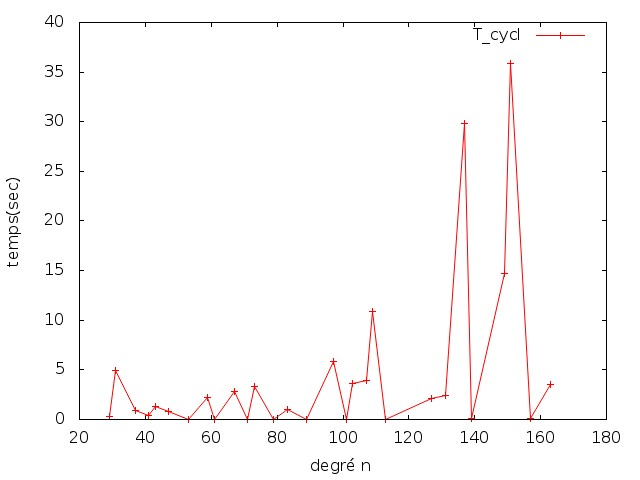
\includegraphics[scale=0.6]{data_test15_testcycl1}
\caption{Temps pour la méthode cyclotomique - caractéristique $p = 101$}
\label{fig:tempscyclopfixed}
\end{center}
\end{figure}

On remarque très clairement que le temps d'exécution est extrêmement variable.
Pour voir la cause de ces pics, il suffit de regarder la valeur de $o$ lors de
l'exécution. Ceci est illustré dans le tableau \ref{tab:resnumcyclavecext}.

\begin{table}[H]
\centering
\begin{tabular}{|c|c|c|}
	\hline
	$n$ & temps (sec) & $o$\\
	\hline
	\hline
	109 & 10.839999 & 5\\
	\hline
	137 & 29.586665 & 6\\
	\hline
	149 & 14.503332 & 4\\
	\hline
	151 & 35.593329 & 6\\
	\hline
\end{tabular}
\caption{Temps d'exécution lorsque $o > 1$}
Méthode cyclotomique
\label{tab:resnumcyclavecext}
\end{table}

Les valeurs de $p$ sont relativement peu élevées, mais si on compare au temps
lorsque $o = 1$ dans le tableau \ref{tab:resnumcyclsansext}, le résultat est 
sans appel. Le problème est donc clairement la construction de l'extension
supplémentaire qui prend énormément de temps. Quant à choisir entre chercher un 
$m$ plus grand ou utiliser une méthode alternative, il faudrait pouvoir pousser 
encore plus les expériences.

\begin{table}[h]
\centering
\begin{tabular}{|c|c|c|}
	\hline
	$n$ & temps (sec) & $o$\\
	\hline
	\hline
	53 & 0.01 & 1\\
	\hline
	79 & 0.02 & 1\\
	\hline
	113 & 0.04 & 1\\
	\hline
	139 & 0.07 & 1\\
	\hline
	157 & 0.096667 & 1\\
	\hline
\end{tabular}
\caption{Temps d'exécutions pour $p = 101$ lorsque que $o = 1$}
Méthode cyclotomique
\label{tab:resnumcyclsansext}
\end{table}
On fixe cette fois-ci le degré $n = 71$ et on fait varier la caractéristique à
partir de $23$, le résultat obtenu est dans la figure \ref{fig:tempscyclnfixed}
\begin{figure}[H]
\begin{center}
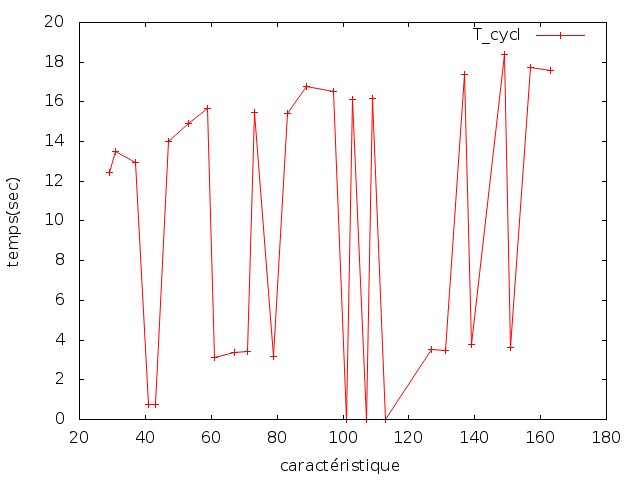
\includegraphics[scale=0.6]{data_test16_testcycl_fixed_degree7}
\caption{Temps d'exécutions - degré $n = 71$ - Méthode cyclotomique}
\label{fig:tempscyclnfixed}
\end{center}
\end{figure}
Bien que la variation globale soit toujours aussi ératique, on remarque deux
lignes plutôt stables correspondant à des valeurs de $o$ fixes. On peut observer
dans les tableaux en annexes \ref{tableau} que à caractéristique fixé $o$ prend
huit valeurs différents, alors qu'à degré fixé, $o$ ne prend que quatre valeurs
différentes.\par
On remarque alors qu'à degré d'extension fixée, le temps d'exécutions évolue
relativement lentement. Ce qui confirme encore une fois le fait que
la gestion des extensions supplémentaires est problèmatique.

\subsection{Méthode elliptique}
On fixe à nouveau $p = 101$, on va maintenant s'intéresser au temps d'éxécution
que prend la méthode elliptique qu'on implanté dans le logiciel \bsc{SAGE}.
Le temps d'exécution complet de la méthode elliptique en fonction du degré est
illustrer dans la figure \ref{fig:tempsellfullpfixed}.\par
\begin{figure}[H]
\begin{center}
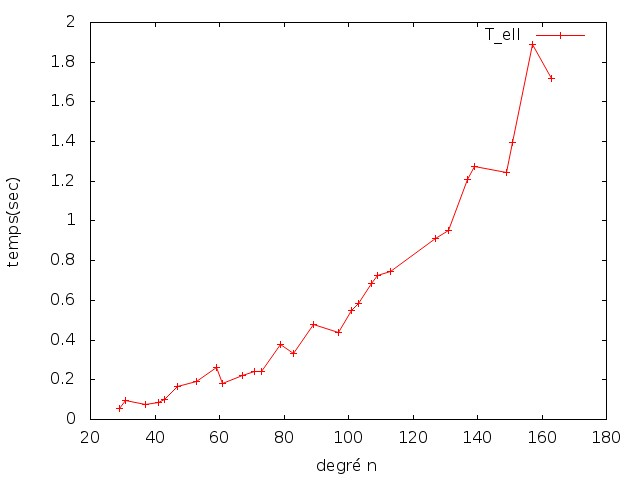
\includegraphics[scale=0.6]{data_test17_testell2}
\caption{Temps d'exécutions - degré $p = 101$ - Méthode elliptique}
\label{fig:tempsellfullpfixed}
\end{center}
\end{figure}
Regardons plus en détails le temps d'exécutions selon chaque partie de
l'algorithme. On rappelle que certains temps donnés dans la figure
\ref{fig:tempsellpartpfixed} sont divisés par deux par rapport à la figure 
\ref{fig:tempsellfullpfixed} puisque ces opérations sont exécutées deux fois
dans le programme.\par
On remarque dans la figure \ref{fig:tempsellpartpfixed} que la partie qui 
demande le plus ressources est la multiplication par un scalaire ou de façon
équivalente le temps qu'il faut pour trouver un point d'ordre $m$.\par
Les temps d'exécution au départ était beaucoup plus catastrophique, il a fallu
travailler cette partie grâce à des formules de Weierstrass $XY$ et utiliser la
bibliothèque \bsc{Flint} afin de pouvoir diminuer le temps d'exécution de cette
fonction.\par
Malheureusement, il semblerait qu'on ne puisse pas diminuer beaucoup plus le
temps d'exécution avec divers optimisation de programmation. À moins de trouver
une amélioration théorique, la multiplication par un scalaire ne pourra pas
arriver à l'ordre de grandeur du temps d'exécution des autres fonctions.
\begin{figure}[H]
\begin{center}
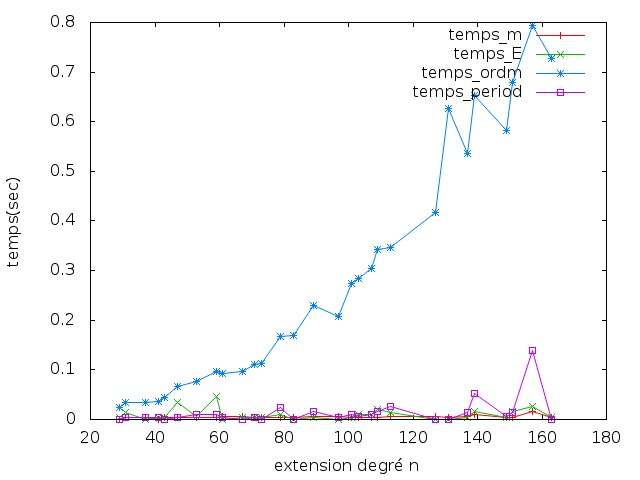
\includegraphics[scale=0.6]{data_test1_p_fixed5}
\caption{Temps d'exécutions - degré $p = 101$ - Méthode elliptique}
\label{fig:tempsellpartpfixed}
\end{center}
\end{figure}
\begin{enumerate}[-]
	\item temps\_m : le temps pour trouver un entier $m$ avec les
bonnes propriétés;
	\item temps\_E : le temps pour trouver une bonne courbe elliptique;
	\item temps\_ordm : le temps pour trouver un point d'ordre $m$ sur
$E/\GF{q^n}$;
 	\item temps\_period : le temps pour calculer les périodes elliptiques.
\end{enumerate}

\subsection{Changement de base}
On fixe $p = 101$ et on va déterminer le temps qu'il faut, une fois après avoir
trouvé deux éléments, pour déterminer l'image de $x$, le générateur de la base
monomiale. Sur la figure, il y a le temps d'exécution pour le calcul des 
coefficients de $x$ dans la base normale (t\_coeff) et et le temps que prend son
écriture dans la base monomiale (t\_isom).
\begin{figure}[H]
\centering
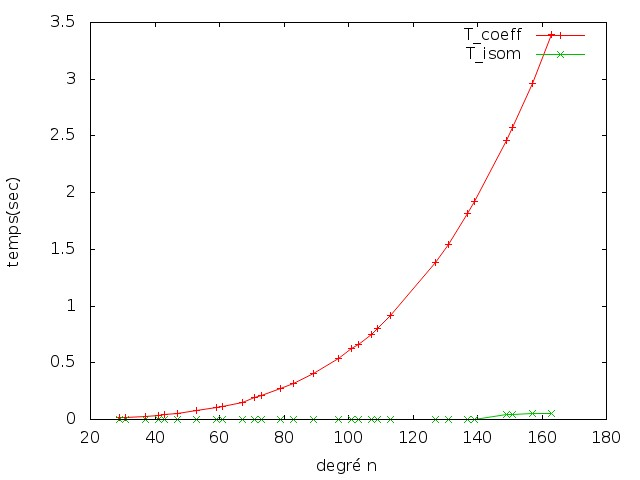
\includegraphics[scale=0.6]{data_test19_testnorm2}
\caption{Temps d'exécution pour $p = 1$ - coefficients dans la base normale}
\label{fig:tempsbasenormale}
\end{figure}
Malheureusement, on voit clairement que la progression du temps semble être
proche de l'exponentielle, ce n'est donc pas une méthode efficace. Heureusement,
il existe d'autres méthodes déduisant l'image de $x$ grâce à deux
éléments reliés dans des temps acceptables.


\section{Comparaison avec d'autres méthodes}
%TODO: 
% - Comparer cyclotomique vs elliptic, avec et sans extensions; !! Une bone idée
% pourrait être de "voir" quelle serait la proportion de premier tel qu'il y
% aurait besoin d'une extension, en fonction de p, en fonction n etc.
%
% - Comparer cyclo vs allombert
%
% - Comparer allombert vs ellpitic
%
% - Comparer détermination de l'isomorphisme entre l'algo de javad et le mien
% (ou bien je le fais avant ?)
Dans la partie théorique, on a pu se rendre compte que toutes les méthodes ont à
peu près la même complexité en $\tO{n^2}$ où $n$ est le degré de l'extension
traité. Nous allons maintenant comparé les différentes méthodes évoquées :
la méthode naïve, la méthode d'Allombert, la méthode de Rains et la variante
elliptique de Rains. On fixe $p = 101$, toutes les mesures seront fait en
fonction du degré.

\begin{figure}[H]
\centering
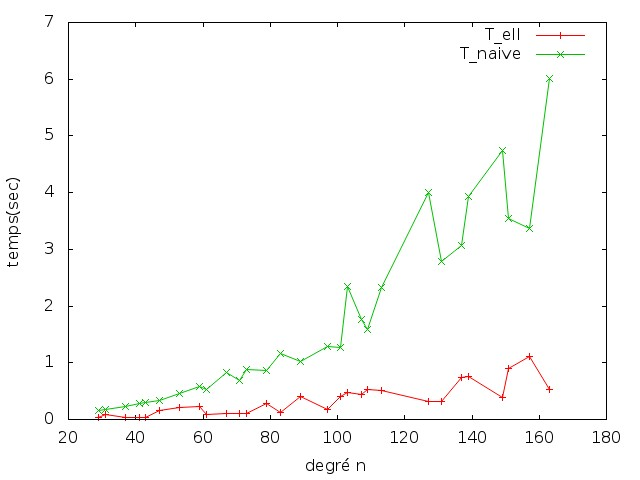
\includegraphics[scale=0.6]{data_test12_cmpellFFH1}
\caption{Comparaison méthode naïve - méthode elliptique}
\label{fig:ellvsnaive}
\end{figure}

Comme le montre la figure \ref{fig:ellvsnaive} nous avons au moins rempli une
partie de notre objectif en implémentant une méthode plus performante que la
méthode naïve exposée au début de la partie \ref{deux}.

\begin{figure}[H]
\centering
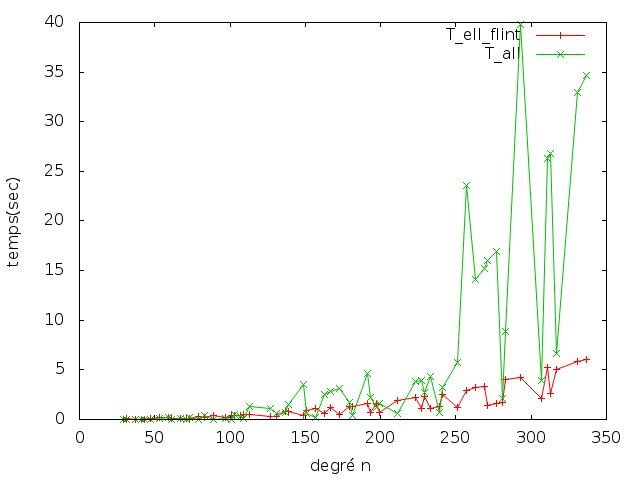
\includegraphics[scale=0.6]{data_test14_cmpellFFH3}
\caption{Comparaison méthode d'Allombert - méthode elliptique}
\label{fig:ellvsallom}
\end{figure}

La figure \ref{fig:ellvsallom} montre qu'asymptotiquement la méthode
elliptique est plus stable que la méthode d'Allombert. Il se peut bien entendu 
que la méthode d'Allombert ait des cas pathologiques similaires à ceux de la 
méthode cyclotomique. Dans ces cas favorables, la méthode d'Allombert est
cependant plus rapide que la méthode ellpitique.


\begin{figure}[H]
\centering
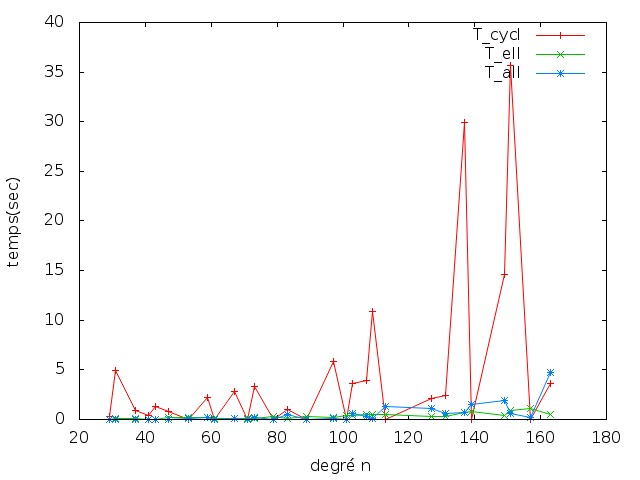
\includegraphics[scale=0.6]{data_test14_cmpellFFH8}
\caption{Comparaison Allombert - elliptique - cyclotomique - $o\geq1$}
\label{fig:ellvsallomvscyclgen}
\end{figure}

Si on ne fixe pas de critère particulier sur les différents paramètres, d'après
la figure \ref{fig:ellvsallomvscyclgen}, on voit clairement que la méthode
cyclotomique peine lorsque $o > 1$; de son côté la méthode d'Allombert ralentit
aussi pendant ces cas pathologiques.

\begin{figure}[H]
\centering
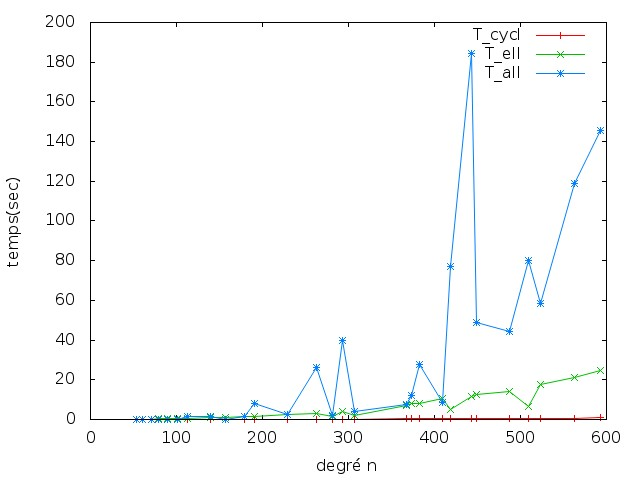
\includegraphics[scale=0.6]{data_test7_flint1}
\caption{Comparaison Allombert - elliptique - cyclotomique - $o=1$}
\label{fig:ellvsallomvscyclsansext}
\end{figure}

Cependant, en imposant alors $o = 1$, la figure 
\ref{fig:ellvsallomvscyclsansext}
montre une domination importante de la méthode cyclotomique.


On observe qu'en moyenne la méthode elliptique sera plus performante que les 
autres méthodes présentées grâce sa relative stabilité. Cependant, si on 
détecte un cas favorable à l'une des deux autres méthodes, leurs performances 
dépassent celle de la méthode elliptique, c'est plus particulièrement le cas 
pour la méthode cyclotomique.\par


\newpage
\part{Conclusion}
\label{quatre}
%TODO: Expliquer ce qu'il peut rester à faire :  car(K) = 2; n  composé; couper 
% et appliquer l'une des deux méthodes selon la nature du m ou s'il y a besoin 
% de calculer une extension, etc.); toute la partie sur la détermination de
% l'isomorphisme (plus profond etc.)
Dans la partie \ref{deux}, nous avons construit une nouvelle variante de 
l'algorithme de Rains, la variante elliptique. D'après les résultats obtenus 
dans la partie \ref{trois}, il se trouve que, contrairement au sentiment premier
de Rains, cette variante est loin d'être sans intérêt. Au contraire, nous avons
pu montrer, au travers de nos expériences, que malgré le fait que les diverses
méthodes aient toutes la même complexité asymptotique, leurs performances sont
en pratique clairement différentes; la méthode elliptique ayant affiché des
performances plus qu'honorables voir compétitives dans certains
cas.\par
Nous avons donc implanter une fonction en \bsc{SAGE} permettant de calculer des 
isomorphismes de corps finis dans un temps raisonnable. Le calcul d'isomorphisme
de corps finis étant une opération courante, il est donc possible, après 
optimisation et regroupement des différentes méhtodes dans une fonction
globale, que le code produit soit intégré dans la bibliothèque de \bsc{SAGE} 
qui ne possède pas encore de telles fonctions.\par

\vspace{0.3cm}

Un autre problème conséquent du calcul d'isomorphismes de corps fini brièvement
traité dans le présent mémoire est la détermination de l'image du générateur de 
la base monomiale. Comme on a pu le voir, si les algorithmes ont des 
performances acceptables pour déterminer deux éléments définissant un iso
morphisme, la solution proposée pour calculer l'image du générateur de la base 
monomiale est quant à elle plutôt médiocre comparée à d'autres algorithmes déjà 
implantés.\par
Il se trouve que c'est un problème riche et qui mérite une attention toute
particulière. On peut imaginer qu'en combinant un algorithme performant
résolvant ce problème et ceux présentés dans ce mémoire, on puisse finalement
résoudre le problème d'isomorphisme dans des temps acceptables; il restera alors
à traiter l'évaluation de cet isomorphisme.
\newpage

\addcontentsline{toc}{part}{Références}
\begin{thebibliography}{LC}

\bibitem{All} \emph{Explicit Computation of Isomorphisms between Finite
Fields}, \bsc{Bill Allombert}, Elsevier Science, 2002, \bsc{url :}
\url{http://www.sciencedirect.com/science/article/pii/S1071579701903442}

\bibitem{CasHen} \emph{The distribution of the number of points modulo an
integer on elliptic curves over finite fields}, \bsc{Wouter Castryck} \&
\bsc{Hendrik Hubrechts}, 2009, \url{http://arxiv.org/abs/0902.44332} 

\bibitem{CouRe} \emph{Elliptic periods for finite fields}, \bsc{Jean-Marc
Couveignes} \& \bsc{Reynald Lercier}, Finite Fields and their Applications,
15(1):1-22, 2009.

\bibitem{Esc} \emph{Théorie de Galois}, \bsc{Jean-Pierre Escofier}, Dunod, 2nde
éd., 2000.

\bibitem{FeGaSho} \emph{Normal Basis \textup{via} General Gauss Periods},
\bsc{Sandra Feisel}, \bsc{Joachim von zur Gathen} \& \bsc{M. Amin Shokrollahi}, 
Mathematics of computation, Volume 68, Number 225, January 1999, p. 271-290.

\bibitem{GaoGaPaSho} \emph{Algorithms for exponentiation in finite fields},
\bsc{Shuhong Gao}, \bsc{Joachim Von Zur Gathen}, \bsc{Daniel Panario} \& 
\bsc{Victor Shoup}, Journal of Symbolic Computation 29:879-889, 2000.

\bibitem{GaGe} \emph{Modern Computer Algebra}, \bsc{Joachim von zur Gathen} \&
\bsc{Jürgen Gerhard}, 3rd edition, Cambridge, 2013.

\bibitem{GaSho} \emph{Computing Frobenius maps and factoring polynomials},
\bsc{Joachim von zur Gathen} \& \bsc{Victor Shoup}, Computational Complexity
2:187-224, 1992.

\bibitem{Lan1} \emph{Algebra}, \bsc{Serge Lang}, Graduate Texts in Mathematics,
3rd ed., Springer, 2005.

\bibitem{Lan2} \emph{Algebraic Number Theory}, \bsc{Serge Lang}, Graduate Texts
in Mathematics, 2nd ed., Springer, 2000.

\bibitem{LiNi1} \emph{Finite Fields}, \bsc{Rudolf Lidl} \& 
\bsc{Harald Niederreiter}, Encyclopedia of mathematics and its applications vol.
20, Cambridge, 1983.

\bibitem{LiNi2} \emph{Introduction to Finite Fields and their Applications},
\bsc{Rudolf Lidl} \& \bsc{Harald Niederreiter}, Cambridge University Press,
1986.

\bibitem{MuPa} \emph{Handbook of Finite Fields}, \bsc{Gary L. Mullen} \& 
\bsc{Daniel Panario}, Discrete mathematics and its applications, Series Editor 
Kenneth H. Rosen, CRC Press.

\bibitem{MiMoScho} \emph{Computing the Eigenvalue in the Schoof-Elkies-Atkin
Algorithm using Abelian Lifts}, \bsc{P. Mih\u{a}ilescu}, \bsc{F. Morain} \&
\bsc{É. Schost}, 2007, \bsc{url :}
\url{http://hal.inria.fr/LIX/inria-00130142/en/}

\bibitem{Per} \emph{Cours d'algèbre}, \bsc{Daniel Perrin}, ellipses, 1996.

\bibitem{Pin} \emph{Recognising Elements of Finite Fields}, \bsc{Richard G.E. 
Pinch}, Cryptography and coding II, p. 193-197, Oxford University Press, 1992.

\bibitem{Rai} \emph{Efficient Computation of Isomorphism Between Finite Fields},
\bsc{Eric M. Rains}, 1996, communication personnelle.

\bibitem{Sam} \emph{Théorie algébrique des nombres}, \bsc{Pierre Samuel}, 
Hermann, 1971.

\bibitem{Scho} \emph{Couting poins on elliptic curves over finite fields},
\bsc{René Schoof}, Journal de théorie des nombres de Bordeaux 7, pp. 219-254,
1995.

\bibitem{Sil} \emph{The Arithmetic of Elliptic Curves}, 
\bsc{Joseph H. Silverman}, Graduate texts in mathematics, Springer, 2nd ed. 
2009.

\bibitem{Was1} \emph{Introduction to Cyclotomic Fields}, \bsc{Lawrence C. 
Washington}, Graduate texts in mathematics, Springer-Verlag, 1982.

\bibitem{Was2} \emph{Elliptic Curves, Number Theory and Cryptography},
\bsc{Lawrence C. Washington}, Chapman \& Hall/CRC, 2nd éd., 2008.

\end{thebibliography}
\newpage
\appendix
\addcontentsline{toc}{part}{\appendixname}
\section{Code}
\label{code}
Tous les programmes sont disponible à l'adresse
\url{https://github.com/defeo/ffisom} et
\url{https://github.com/jpflori/sagemath/tree/ffisom/src/sage/ffisom}.\\
Pour les implémentations, on a utilisé les codes regroupés dans le second
lien.\\
Les routines de tests (non documentées au moment de la rédaction) sont 
disponibles à l'adresse suivante :
\url{https://github.com/brieulle/Rains-pinch/tree/master/gnutests} et nécessite 
l'utilisation de la version sage disponible ici : 
\url{https://github.com/jpflori/sagemath/}

\section{Tableaux de résultats}
\label{tableau}
\begin{table}[H]
\centering
\begin{tabular}{|c|c|c|}
\hline
$n$ & temps(sec) & $o$\\
\hline
\hline
29 & 0.290001&  2\\
\hline
31&  4.956666 & 10\\
\hline
37&  0.933333 & 4\\
\hline
41 & 0.393333 & 2\\
\hline
43 & 1.33 & 4\\
\hline
47 & 0.793333&  3\\
\hline
53 & 0.01 & 1\\
\hline
59 & 2.236666 & 4\\
\hline
61 & 0.013333 & 1\\
\hline
67 & 2.823333 & 4\\
\hline
71 & 0.016667 & 1\\
\hline
73 & 3.29 & 4\\
\hline
79 & 0.016667 & 1\\
\hline
83 & 0.973334 & 2\\
\hline
89 & 0.023334 & 1\\
\hline
97 & 5.796667 & 4\\
\hline
101 & 0.03 & 1\\
\hline
103 &3.63& 3\\
\hline
107 & 3.916666 & 3\\
\hline
109 & 10.929999 & 5\\
\hline
113 & 0.04 & 1\\
\hline
127 & 2.133333 & 2\\
\hline
131 & 2.383333 & 2\\
\hline
137 & 29.83333 & 6\\
\hline
139  &0.07 & 1\\
\hline
149 & 14.663332 & 4\\
\hline
151  &35.849997 & 6\\
\hline
157 & 0.096666 & 1\\
\hline
163 & 3.499999 & 2\\
\hline
\end{tabular}
\caption{Résultats complets de la figure \ref{fig:tempscyclopfixed}}
\end{table}


\begin{table}[H]
\centering
\begin{tabular}{|c|c|c|}
\hline
$p$ & temps (sec)& $o$\\
\hline
\hline
29 &12.449999& 8\\
\hline
31 &13.523332& 8\\
\hline
37 &12.956666& 8\\
\hline
41 &0.773333& 2\\
\hline
43 &0.766667& 2\\
\hline
47 &13.979999& 8\\
\hline
53 &14.916665 &8\\
\hline
59 &15.669998 &8\\
\hline
61 &3.143334& 4\\
\hline
67 &3.369999& 4\\
\hline
71 &3.429999 &4\\
\hline
73 &15.466665 &8\\
\hline
79 &3.193333& 4\\
\hline
83 &15.396665& 8\\
\hline
89 &16.769999& 8\\
\hline
97 &16.543332& 8\\
\hline
101& 0.02& 1\\
\hline
103& 16.123331& 8\\
\hline
107& 0.016667 &1\\
\hline
109& 16.189998& 8\\
\hline
113& 0.016667 &1\\
\hline
127& 3.533333 &4\\
\hline
131& 3.493332 &4\\
\hline
137& 17.376665& 8\\
\hline
139& 3.773333 &4\\
\hline
149& 18.376664& 8\\
\hline
151& 3.619999 &4\\
\hline
157& 17.753332& 8\\
\hline
163& 17.593332& 8\\
\hline
\end{tabular}
\caption{Résultats complets de la figure \ref{fig:tempscyclnfixed}}
\end{table}
\end{document}

